\documentclass[10pt]{beamer}

\mode<presentation>
{
 \usetheme{Boadilla}
\pagestyle{empty}

\setbeamerfont*{frametitle}{size=\normalsize,series=\bfseries}
\setbeamerfont*{block}{size=\normalsize,series=\bfseries}
%\setbeamertemplate{blocks}[rounded][shadow=true]
}

\definecolor{links}{HTML}{2A1B81}
\hypersetup{colorlinks,linkcolor=,urlcolor=links}


\usepackage[pdf]{pstricks}
\usepackage{pst-sigsys}


\definecolor{darkblue}{rgb}{0.0, 0.0, 0.40}
\setbeamercolor{title}{fg=darkblue}
\setbeamercolor{frametitle}{fg=darkblue}
\definecolor{darkgreen}{rgb}{0.0, 0.4, 0.0}

\usepackage{bbm}
\usepackage{etex}
% \usepackage{helvet}
\usepackage{amsmath, amssymb}
\usepackage{color}
\usepackage{asymptote}
\usepackage{mathrsfs}
\usepackage{dsfont}
\usepackage{makeidx}
\usepackage{multido}

\usepackage{pst-sigsys,pst-plot,pstricks-add}
%\usepackage{auto-pst-pdf}
\usepackage{pst-pdf}

\usepackage[american voltages, american currents,siunitx]{circuitikz}

\definecolor{links}{HTML}{2A1B81}
\hypersetup{colorlinks,linkcolor=,urlcolor=links}

\def\nn{\nonumber}

\definecolor{links}{HTML}{2A1B81}
\hypersetup{colorlinks,linkcolor=,urlcolor=links}

\newcommand{\fs}[2]{#2}

\title[]{Introduction to Electric Circuits. \\ Basic Magnitudes and Elements. Kirchhoff's Laws.}
\author[\textcolor{blue}{Systems and Circuits}]{\textcolor{darkblue}{Pablo M. Olmos} (olmos@tsc.uc3m.es)\\ \textcolor{darkblue}{Emilio Parrado} (emipar@tsc.uc3m.es)}
\institute{\textcolor{white}{UC3M}}

\AtBeginSection[]
{
  \begin{frame}<beamer>{Index}
    \tableofcontents[currentsection,currentsubsection]
  \end{frame}
}

\begin{document}
\frame{
\titlepage
\thispagestyle{empty}
\begin{center}

\includegraphics[scale=0.05]{Figures/uc3m-logo.pdf}
\end{center}
}


\frame{




\begin{itemize}
\item An electric circuit is composed of individual components connected by conductive wires or traces through which \textbf{electric current can flow}. 
\end{itemize}
\begin{itemize}
\item The combination of components and wires allows various simple and complex operations to be performed: signals can be amplified, computations can be performed, and data can be moved from one place to another.
\end{itemize}


%\begin{center}
%\begin{pspicture}[](5,2)
%   \pssignal(0,1){x}{Input Signal}
%   \psblock(4,1){a}{Electric Circuit}
%   %\psblock(4,1){b}{$h[n], H(z)$}
%   \pssignal(8,1){y}{Output Signal}
%   %-----------------
%   \psset{arrows=->}
%   \ncline{x}{a}  \ncline{a}{y}  %\ncline{b}{y}
%\end{pspicture}
%\end{center}
}

\frame{

\begin{figure}
\centering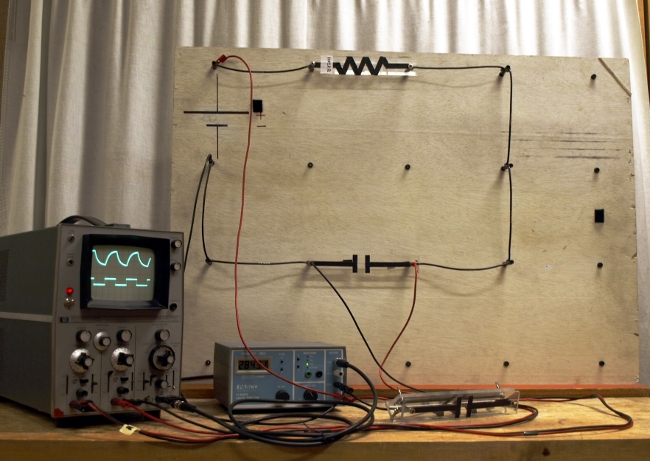
\includegraphics[scale=0.4]{Figures/RC_circuit_setup.jpg}
\caption{Rudimentary setting for an electric circuit containing one battery, one resistor and one capacitor. In the oscilloscope, we observe the input/output voltage signals (bottom and top signals respectively).}
\end{figure}

}

\frame{
In  this course:
\begin{itemize}
\item Basic analysis  tools.
\item Passive Electric circuits: Resistors+Capacitators+Inductions $\Rightarrow$ \textbf{\underline{filters}}.
\begin{figure}
\centering\includegraphics[scale=0.5]{Figures/filters.pdf}
\end{figure}
\item Application of  concepts on signal \& systems.
\end{itemize}

\begin{exampleblock}{}
We assume you have had an introductory physics course in which the electrical and magnetic phenomena were discussed.
\end{exampleblock}

}

\frame{
\frametitle{Recommended books}
\begin{itemize}
\item Electric circuits, James William Nilsson.
\item Principles of Electric Circuits, Thomas Floyd.
\end{itemize}

}


\section{Introduction to Circuit Theory.}

\frame{
\frametitle{Circuit Theory}
\begin{itemize}
\item Circuit theory is a special case of electromagnetic field theory, i.e., the study of static and moving electric charges.
\item Applying the general electromagnetic field theory to investigate electrical circuits  is cumbersome and requires the use of advanced mathematics.
\item In circuit theory, we rely on three physical assumptions:
\end{itemize}
\begin{block}{}
In circuit theory we ignore the propagation effects of the electrical signals throughout the circuit. Electrical effects happens instantaneously.
\end{block}
\begin{exampleblock}{}
The net charge on every component in the system is always zero.  No component can collect a net excess of charge. 
\end{exampleblock}
\begin{alertblock}{}
There is no magnetic coupling between the components in a system.
\end{alertblock}

}

\frame{
\frametitle{Circuit Theory}
This approach yields the following benefits:
\begin{enumerate}
\item Circuit theory provides \textbf{simple solutions} (of sufficient accuracy) to problems that are prohibitively complex by applying the general theory. 
\item \textbf{Divide and conquer approach:} subsystems called components are first analyzed. We can use the behavior of each component to predict the behavior of bigger systems.
\item Circuits analysis introduces a \textbf{methodology for solving large networks of coupled linear equations}, which are prevalent through engineering and technology.
\end{enumerate}

}

\section{Basic magnitudes and elements.}

\frame{
\frametitle{Electrical Charge}

\begin{itemize}
\item Property of matter: excess or deficiency of electrons. We symbolize the charge by $Q$.
\item The electric charge exists in discrete quantities. The electron is the smallest particle that exhibits negative electrical charge.
\item Coulomb is the unit of charge. $Q_e=-1.6 10^{-19}$ C.
\item The charge of the proton is equal in magnitude to the electron charge, but with opposite sign.
\end{itemize}

\begin{exampleblock}{Circuit theory}
Electrical effects are attributed to both the separation of charges, which creates \textbf{ an electrical force (voltage)}, and charges in motion, which creates an \textbf{electric fluid or current}).
\end{exampleblock}

}

\frame{
\frametitle{Voltage}
\begin{itemize}
\item When we separate positive and negative charges, an energy transferred to the charges. 
%\item They have now have the potential to flow across the circuit. 
\item If it is physically possible, charges will move across the circuit until they reach a point with minimum energy.
\item The voltage between two points of the circuit is the difference of electrical energy per unit charge between the two points.
\end{itemize}

\begin{alertblock}{The energy is never lost, just transformed. }
When we separate charges we transform chemical energy (a battery) into electrical energy. When charges flow throughout the circuit, the electrical energy that they lose is transformed into a different kind of energy, e.g., heat in the case of a heater or light in the case of a lamp.
\end{alertblock}

}

\frame{

\begin{block}{Voltage}
Energy per unit charge:
\begin{align}\nonumber 
V=\frac{\partial W}{\partial Q}\qquad \text{volts (V)}
\end{align}
One volt is the potential difference between two points when one joule of energy is used to move one coulomb of positive charge from one point to the other.  
\end{block}

}


\frame{
\frametitle{Electrical current}

\begin{itemize}
\item Under normal conditions the movement of the electrons is truly random, meaning they are moving in all directions by the same amount.
\item If a voltage is placed across a conductive material, it causes the free electrons to move in a single direction. 
\item We define the electrical current as the rate of charge flow past a given point in an electric circuit:
\begin{align}\nonumber
I(t)=\frac{\partial Q}{\partial t} \qquad \text{Amperes (A)}
\end{align}


\end{itemize}

\begin{columns}
\begin{column}{0.5\textwidth}
\begin{figure}
\centering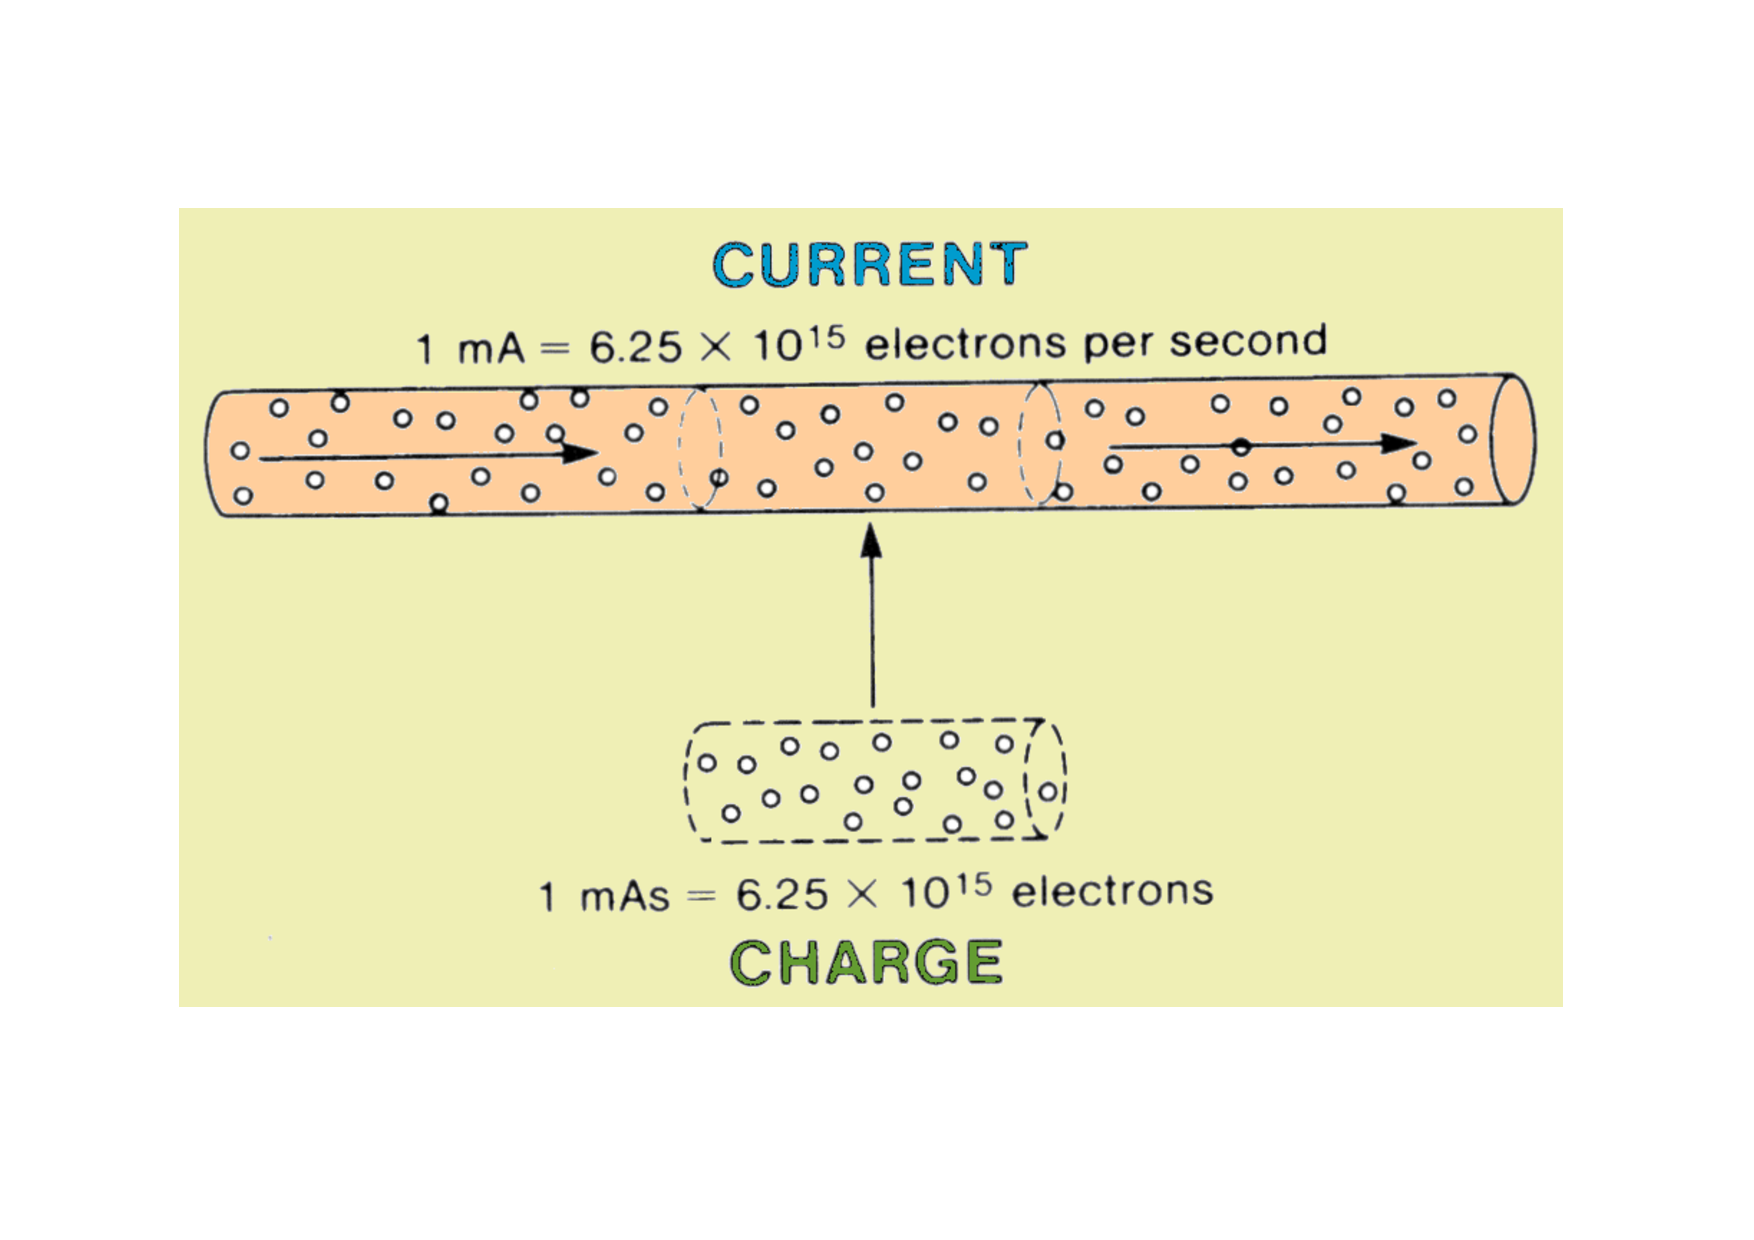
\includegraphics[scale=0.25]{Figures/current.pdf}
\end{figure}
\end{column}
\begin{column}{0.5\textwidth}
\begin{block}{}
One ampere is the amount of current that exists when a number of electrons having a total charge of one coulomb move trough a given cross-sectional area in one second.
\end{block}
\end{column}
\end{columns}

}

\frame{
\frametitle{The Ideal Basic Circuit Element}

\begin{columns}
\begin{column}{0.35\textwidth}
\begin{center}
\begin{circuitikz} \draw 
  (0,-1) to[generic] (0,1)
  (2,1) to[short,i=$i$](0,1)
  (0,-1) to[short] (2,-1)
  node[ocirc] (A) at (2,1) {}
  node[ocirc] (B) at (2,-1) {}
 (A) to[open, v=$v$] (B)
 (-0.5, 1) node[anchor=east]{A}
 (-0.5, -1) node[anchor=east]{B};
\end{circuitikz}
\end{center}
\end{column}
\begin{column}{0.65\textwidth}
\begin{alertblock}{}
Any element will be defined by a certain $v=f(i)$ function. 
\end{alertblock}
\end{column}
\end{columns}
\begin{exampleblock}{}
The voltage across the terminals $A-B$ is denoted by $v$. We  arbitrarily assume $A$ as the positive terminal $(+)$ and $B$ as the negative terminal $(-)$.
\end{exampleblock}

\begin{itemize}
\item If $v>0$, \textbf{positive charges} in $A$ have more energy than in $B$. 
\item If $v<0$, \textbf{positive charges} in $B$ have more energy than in $A$. 
\item \textbf{Conventional current flow:} we consider the current as a flow of positive charges.
\end{itemize}



}

\frame{

\begin{center}
\begin{circuitikz} \draw 
  (0,-1) to[generic] (0,1)
  (2,1) to[short,i=$i$](0,1)
  (0,-1) to[short] (2,-1)
  node[ocirc] (A) at (2,1) {}
  node[ocirc] (B) at (2,-1) {}
 (A) to[open, v=$v$] (B)
 (-0.5, 1) node[anchor=east]{A}
 (-0.5, -1) node[anchor=east]{B};
\end{circuitikz}
\end{center}

\begin{itemize}
\item $v=5$v and $i=2$A $\rightarrow$ current flows from a point of where charges have more energy $(A)$ to a point where they have less energy $(B)$. \textbf{The device is consuming electrical energy.}
\item $v=5$v and $i=-2A$ $\rightarrow$ current flows from a point of where charges have less energy $(B)$ to a point where they have more energy $(A)$. \textbf{The device is generating electrical energy.} E.g., it is a battery.
\end{itemize}


}

\frame{
\frametitle{Electric Power}

\begin{itemize}
%\item Assume a voltage $V(t)$ between both extremes of a two-terminal device in an electric circuit and a given current $I(t)$ moving throughout it.
\item Electric power $P(t)$ is the amount of electric energy $W(t)$ consumed/generated used per unit time:
\begin{align}\nonumber
P(t)=V(t)I(t) \qquad \text{Watts (W)}
\end{align} 
\end{itemize}

\begin{exampleblock}{}
\begin{columns}
\begin{column}{0.35\textwidth}
\begin{circuitikz} \draw 
  (0,-1) to[generic] (0,1)
  (2,1) to[short,i=$i$](0,1)
  (0,-1) to[short] (2,-1)
  node[ocirc] (A) at (2,1) {}
  node[ocirc] (B) at (2,-1) {}
 (A) to[open, v=$v$] (B)
 (-0.5, 1) node[anchor=east]{A}
 (-0.5, -1) node[anchor=east]{B};
\end{circuitikz}
\end{column}
\begin{column}{0.65\textwidth}
\begin{itemize}
\item If $v>0$ and $i>0$, the charges are losing electrical energy (the device is transforming electrical energy into another kind of energy), thus $P(t)>0$.
\end{itemize}
\end{column}
\end{columns}
\end{exampleblock}

} 

\frame{
\frametitle{Electric Power}

\begin{exampleblock}{}
\begin{columns}
\begin{column}{0.35\textwidth}
\begin{circuitikz} \draw 
  (0,-1) to[generic] (0,1)
  (2,1) to[short,i=$i$](0,1)
  (0,-1) to[short] (2,-1)
  node[ocirc] (A) at (2,1) {}
  node[ocirc] (B) at (2,-1) {}
 (A) to[open, v=$v$] (B)
 (-0.5, 1) node[anchor=east]{A}
 (-0.5, -1) node[anchor=east]{B};
\end{circuitikz}
\end{column}
\begin{column}{0.65\textwidth}
\begin{itemize}
\item If $v>0$ and $i<0$, the element is providing the charges with electrical energy, thus $P(t)<0$.
\end{itemize}
\end{column}
\end{columns}
\end{exampleblock}


\begin{block}{}
Any device that generates power is said to be active (e.g. a voltage source) and otherwise passive (a resistor).
\end{block}
}

\section{Basic circuit elements}

\frame{
\frametitle{Ideal Voltage source}

\begin{center}
\begin{circuitikz} \draw 
  (0,0) to[V=$V_s$] (0,2)
  (2,2) to[short,*-](0,2)
  (0,0) to[short,-*](2,0)
  (3,2) node[anchor=east] {A}
  (3,0) node[anchor=east] {B}
   (6,1) node[anchor=east] {$V_s=V_A-V_B$};
%       to[R=1<\ohm>] (2,2) 
%        to[C=1<\farad>] (2,0) -- (0,0);
\end{circuitikz}
\end{center}

\begin{block}{}
An ideal voltage source maintains a fixed voltage across its terminals $V_s$ regardless of the current $i_s$ in the device.
\end{block}

%\begin{alertblock}{}
%If $V_s>0$, the current $i_s$ flows from the negative terminal $(B)$ to the positive one $(A)$, i.e. $i_s<0$. The device is providing electrical energy to  charges, thus $P=V_s i_s<0$.
%\end{alertblock}

}

\frame{
\frametitle{Voltage sources in series}

\begin{block}{}
When two or more voltage sources are in series, the total voltage is equal to the algebraic sum of the individual source voltages (take care with the polarities!).
\end{block}

\begin{columns}
\begin{column}{0.5\textwidth}
\begin{center}
\begin{circuitikz} \draw 
  (0,0) to[V=$V_1$] (0,1.5)
  to[V=$V_2$](0,3)
  to[V=$V_3$](0,4.5)
  to[short,-*](2,4.5)
  (0,0) to[short,-*] (2,0)
  (2.5,4.5) node[anchor=east] {$A$}
  (2.5,0) node[anchor=east] {$B$}
  (3,-1) node[anchor=east] { $\color{blue}{V_A-V_B=V_1+V_2+V_3}$};
\end{circuitikz}
\end{center}
\end{column}
\begin{column}{0.5\textwidth}
\vspace{0.3cm}

\begin{circuitikz} \draw 
  (0,0) to[V=$V_1$] (0,1.5)
  (0,3) to[V=$V_2$](0,1.5)
  (0,3) to[V=$V_3$](0,4.5)
  to[short,-*](2,4.5)
  (0,0) to[short,-*] (2,0)
  (2.5,4.5) node[anchor=east] {$A$}
  (2.5,0) node[anchor=east] {$B$}
  (3,-1) node[anchor=east] { $\color{blue}{V_A-V_B=V_1-V_2+V_3}$};
\end{circuitikz}
\end{column}
\end{columns}

}


\frame{
\frametitle{Ideal current source}

\begin{center}
\begin{circuitikz} \draw 
  (0,0) to[I] (0,2)
  to[short,o-*](2,2)
  (0,0) to[short,o-*](2,0)
  (-0.5,1) node[anchor=east] {$I_s$};
%       to[R=1<\ohm>] (2,2) 
%        to[C=1<\farad>] (2,0) -- (0,0);
\end{circuitikz}
\end{center}

\begin{block}{}
An ideal current source maintains a fixed current $I_s$ within its terminals  regardless of the voltage across them.
\end{block}

}



\frame{
\frametitle{Current sources in parallel}

\begin{block}{}
The total current produced by current sources in parallel is equal to the algebraic sum of the individual current sources.
\end{block}

\begin{center}
\begin{circuitikz} \draw 
  (0,0) to[I=$I_1$] (0,2)
  to[short](6,2)
  (0,0) to[short](6,0)
  (2,0) to[I=$I_2$] (2,2)
  (4,0) to[I=$I_3$] (4,2)
  (6,2) to[generic] (6,0);
\end{circuitikz}
\end{center}

\begin{center}
\begin{circuitikz} \draw 
  (0,0) to[I=$I_1+I_2+I_3$] (0,2)
  to[short](2,2)
  to [generic] (2,0)
  (0,0) to[short](2,0);
\end{circuitikz}
\end{center}
}

\frame{
\frametitle{Forbidden configurations!}

\begin{columns}
\begin{column}{0.5\textwidth}
\begin{center}
\begin{circuitikz} \draw 
  (0,0) to[V=$V_1$] (0,2)
  to[short](4,2)
  (0,0) to[short](4,0)
  (2,0) to[V=$V_2$] (2,2)
  (4,2) to[generic] (4,0);
\end{circuitikz}
\end{center}
\end{column}

\begin{column}{0.5\textwidth}
\begin{circuitikz} \draw 
  (0,0) to[I=$I_1$] (0,1.5)
   to[I=$I_2$](0,3)
  to[short](2,3)
  (0,0) to[short] (2,0)
  (2,0) to[generic] (2,3);
\end{circuitikz}
\end{column}
\end{columns}

%\begin{exampleblock}{}
%Don't try in the Lab....
%\end{exampleblock}

}

\frame{
\frametitle{Dependent voltage/current sources}

\begin{itemize}
\item The value of the voltage/current generated depends on another magnitude (current/voltage) in the circuit.
\end{itemize}

\begin{center}
\begin{tabular}{cc}
\begin{circuitikz} \draw 
  (0,0) to[cV=$a V_x$] (0,2);
\end{circuitikz}
& 
\begin{circuitikz} \draw 
  (0,0) to[cV=$b I_x$] (0,2);
\end{circuitikz}
\\
\begin{circuitikz} \draw 
  (0,0) to[cI=$c V_x$] (0,2);
\end{circuitikz}
& 
\begin{circuitikz} \draw 
  (0,0) to[cI=$d I_x$] (0,2);
\end{circuitikz}
\end{tabular}
\end{center}

Where $a,b,c,d$ are real constants and $V_x$ and $I_x$ are some voltage/current in the circuit.


}

\frame{
\frametitle{Resistance}

\begin{itemize}
\item When there is current through a material, the free electrons move through the material and occasionally collide with atoms.
\item Collitions cause the electrons to lose some of their energy and the movement is restricted.
\item The property of a material that restrict the flow of electrons is called resistance $R$, measured in Ohms (1$\Omega$).
\end{itemize}

\begin{columns}
\begin{column}{0.5\textwidth}
\begin{figure}
\centering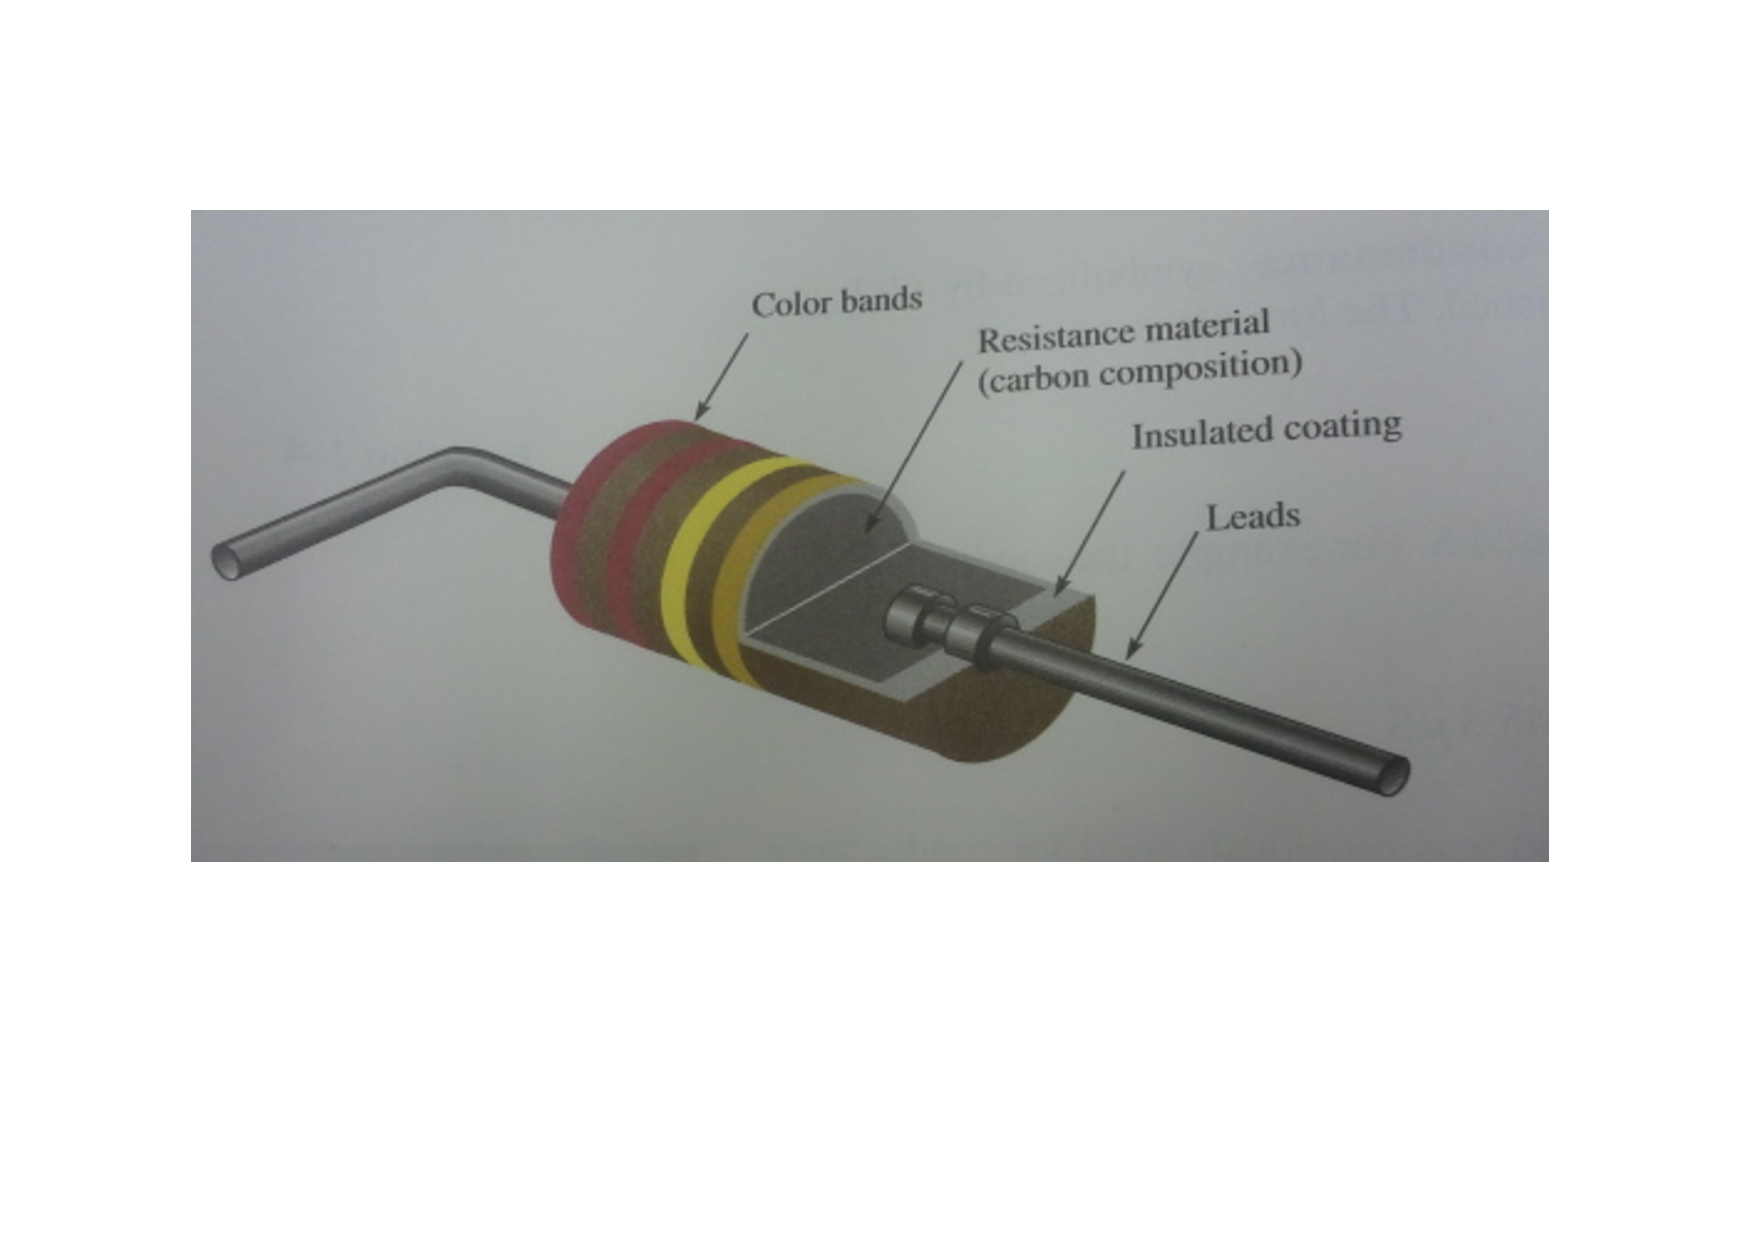
\includegraphics[scale=0.25]{Figures/resistor.pdf}
\end{figure}
\end{column}
\begin{column}{0.5\textwidth}
\begin{block}{}
One ohm (1 $\Omega$) of resistance exists if there is one ampere (1 A) of current in a material when one volt (1 V) is applied across the material.
\end{block}
\end{column}
\end{columns}
\vspace{0.5cm}

\textbf{\color{red}{A resistor is a component that is specifically designed to have a certain amount of resistance.}}

}


\frame{
\frametitle{The Ohm's law}

\begin{block}{}
The current $i(t)$ going through a given resistor is directly proportional to voltage $v(t)$ and inversely proportional to the resistance R:
\begin{align}\nonumber
i(t)=\frac{v(t)}{R}
\end{align}
\end{block}
\vspace{0.5cm}

\begin{columns}
\begin{column}{0.5\textwidth}
\begin{center}
\begin{circuitikz}\draw 
  (1,2) to[short,i=$i(t)$,*-] (2,2)
  to[R=$R$,v<=$v(t)$] (2,0)
  to[short,-*](1,0);
\end{circuitikz}
\end{center}
\end{column}
\begin{column}{0.5\textwidth}
\textbf{The device always consumes power:}
\begin{align*}
P(t)=v(t)i(t)=\frac{v^2(t)}{R}=R i^2(t)>0 \text{   Watt.  }
\end{align*}
\end{column}
\end{columns}

}

\frame{
\frametitle{A very simple circuit}
\begin{center}
\begin{circuitikz}\draw 
  (0,0) to[V=$v_s$] (0,2)
   to[short,i=$i$] (2,2)
  to[R=$R$,v<=$v$] (2,0)
  to[short](0,0);
\end{circuitikz}
\end{center}
\begin{itemize}
\item The voltage sources provides electrical energy to the charges that flow across the resistor.

\end{itemize}
\begin{exampleblock}{Resistor perspective}
The voltage across terminals is $v_s$ and the current is  $i=v_s/R$ (positive, it enters through the positive terminal). Power consumed: $P=v^2_s/R$ Watt.
\end{exampleblock}

\begin{exampleblock}{Voltage source perspective}
The voltage across terminals is $v_s$ and the current is $i=v_s/R$. The power consumed is $P=-v^2_s/R$ Watt (the current enters through the negative terminal of the voltage source). 
\end{exampleblock}
}

\section{Kirchhoff's Laws}

\frame{
\frametitle{Kirchhoff's Laws}
\begin{itemize}
\item A circuit is said to be solved when the voltage across and the current in every element in the circuit have been determined.
\item The interconnection of elements imposes constraints on the relationships between the terminal voltages and currents.
\item These constraints are referred to as Kirchhoff's Laws.
\end{itemize}


}

\frame{
\frametitle{Branches, Loops and nodes}

\begin{itemize}
\item Branch: any element of two terminals (wires do not count).
\item Loop: any set of branches that form a closed loop.
\item Minimal loop: any loop that does not contain another loop.
\item Node: a node is any point where two or more branches are connected.
\item Essential Nodes: any node where at least three branches are connected.
\end{itemize}

\begin{figure}
\centering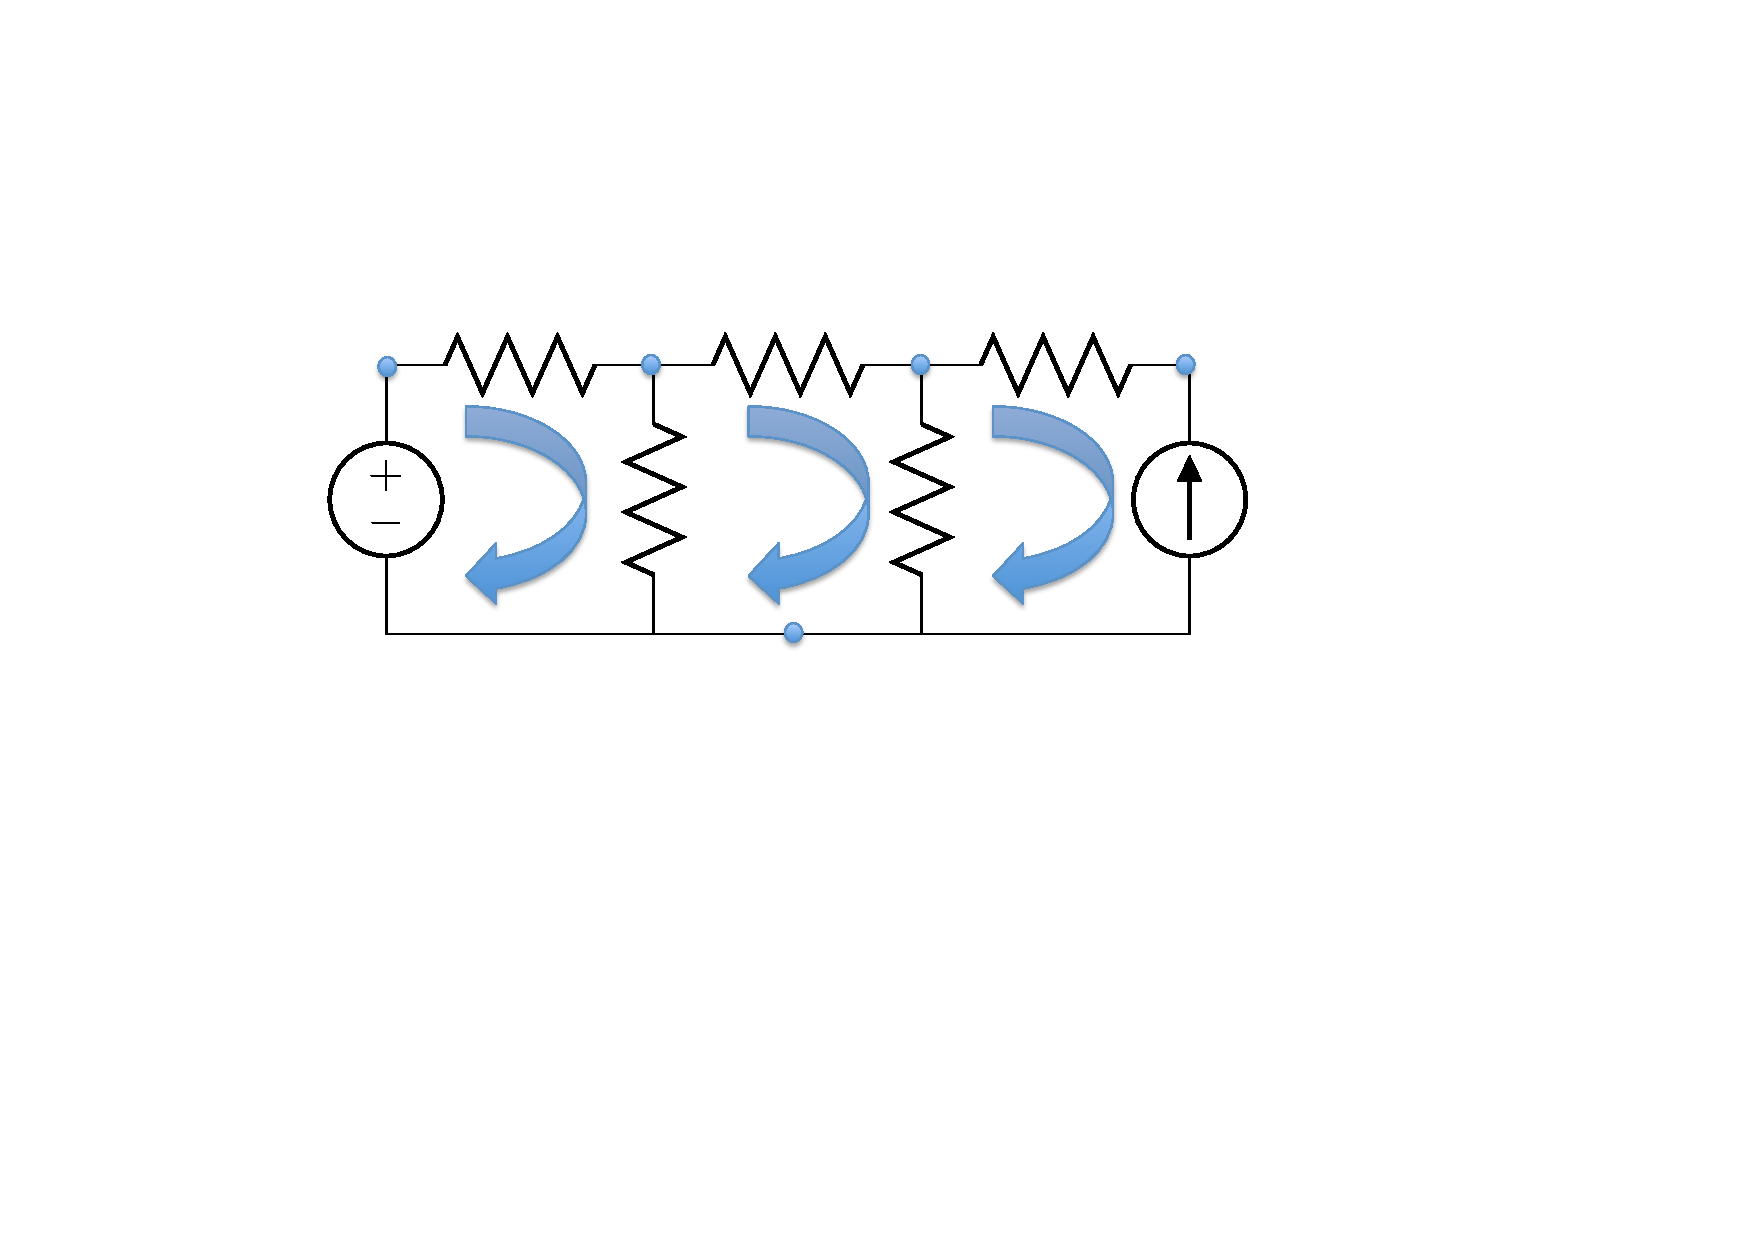
\includegraphics[scale=0.5]{Figures/loops_nodes.pdf}
\caption{7 devices or branches, 3 minimal loops, 5 nodes and 3 essential nodes.}
\end{figure}
}

\frame{
\frametitle{Kirchhoff's current law}

\begin{block}{}
The sum of currents entering any node is equal to the sum of currents leaving that node.
\end{block}


\begin{center}
\begin{circuitikz} \draw 
  (0,0) to[V=$V_s$] (0,2)
  to[short,-*,i=$I_s$](1,2)
  to[short](1,1)
  to[short](1,3)
  (1,2) to[R=$R_2$,i=$I_2$](3,2)
  to[short,*-,i=$I_s$](4,2)
  (1,1) to[R=$R_1$,i=$I_1$](3,1)
    to[short](3,2)
  (1,3) to[R=$R_3$,i=$I_3$](3,3)
    to[short](3,2)
   (4,2) to[short](4,0)
    to[short](0,0)
   (1.05,1.80) node[anchor=east] {A}
   (3.45,1.80) node[anchor=east] {B};
\end{circuitikz}
\end{center}

\begin{columns}
\begin{column}{0.5\textwidth}
\textbf{In node A}
\begin{align}\nonumber
\underbrace{I_s}_{\text{Current in}}=\underbrace{I_1+I_2+I_3}_{\text{Current out}}
\end{align}
\end{column}
\begin{column}{0.5\textwidth}
\textbf{In node B}
\begin{align}\nonumber
\underbrace{I_1+I_2+I_3}_{\text{Current in}}=\underbrace{I_s}_{\text{Current out}}
\end{align}
\end{column}
\end{columns}



}


\frame{
\frametitle{Kirchhoff's voltage law}
\begin{block}{}
In a single closed path, the sum of all the voltage drops must be equal to the sum of the voltage rises.
\end{block}

\begin{columns}
\begin{column}{0.5\textwidth}
\begin{center}
\begin{circuitikz} \draw 
  (0,-1) to[V=$V_s$,i=$I_s$] (0,5)
  to[short](2,5)
  to[short](2,4.9)
  %[european voltages]
  (2,4.89) to[R=$R_1$,v=$V_1$](2,3)
  to[R=$R_2$,v=$V_2$](2,1)
  to[R=$R_3$,v=$V_3$](2,-1)
  to[short](0,-1);
\end{circuitikz}
\end{center}
\end{column}
\begin{column}{0.5\textwidth}
\begin{align}\nonumber
V_s=V_1+V_2+V_3
\end{align}
%\begin{block}{}
%Basic tools to analyze resistive circuits: Kirchhoff's laws + Ohm's law.
%\end{block}
\end{column}
\end{columns}

}

\frame{
\frametitle{Kirchhoff's voltage law}

Another  way to express Kirchhoff's voltage law is as follows:
\begin{block}{}
The algebraic sum of all the voltage drops around a single closed path in a circuit is zero. 
\end{block}

\begin{columns}
\begin{column}{0.5\textwidth}
\begin{center}
\begin{circuitikz} \draw 
  (0,-1) to[V=$V_s$,i=$I_s$] (0,5)
  to[short](2,5)
  to[short](2,4.9)
  %[european voltages]
  (2,4.89) to[R=$R_1$,v=$V_1$](2,3)
  to[R=$R_2$,v=$V_2$](2,1)
  to[R=$R_3$,v=$V_3$](2,-1)
  to[short](0,-1);
\end{circuitikz}
\end{center}
\end{column}
\begin{column}{0.5\textwidth}
We follow the current direction and we algebraically sum the voltage drops. A voltage source represents a negative drop. 
\begin{align}\nonumber
V_1+V_2+V_3\color{red}{-V_s}=\color{black}{0}
\end{align}
\end{column}
\end{columns}

}

\section{Analysis of simple resistive circuits}

\frame{
\frametitle{Compute $i_s$ and the voltage drop in every resistor}


\begin{center}
\begin{circuitikz} \draw 
(0,0) to[V=$V_s$,i=$i_s$] (0,2)
to[R=$R_1$] (2,2)
to[R=$R_2$] (4,2)
to[short](4,0)
to[R=$R_3$] (2,0)
to[short] (0,0);
\end{circuitikz}
\end{center}


}

\frame{
\frametitle{Compute the current across $R_2$}

\begin{center}
\begin{circuitikz} \draw 
  (0,0) to[V=$v_s$,i=$i_s$] (0,2)
  to[short](4,2)
  (0,0) to[short](4,0)
  (2,0) to[R=$R_1$] (2,2)
  (4,0) to[R=$R_2$] (4,2);
\end{circuitikz}
\end{center}


}


\frame{
\frametitle{Compute the power generated by the voltage source}

\begin{center}
\begin{circuitikz} \draw 
  (0,0) to[V=$v_s$] (0,2)
  to[short](6,2)
  (0,0) to[short](6,0)
  (2,0) to[R=$R_1$] (2,2)
  (4,0) to[R=$R_2$] (4,2)
  (6,2) to[R=$R_3$] (6,0);
\end{circuitikz}
\end{center}

}


\frame{
\frametitle{Compute the voltage drop in $R_2$}

\begin{center}
\begin{circuitikz} \draw 
  (0,0) to[V=$v_s$] (0,2)
  to[R=$R_1$](4,2)
  to[R=$R_2$](4,0)
  to[short] (0,0);
\end{circuitikz}
\end{center}

}




%
%%
%%\frame{
%%\frametitle{Atomic Structure}
%%
%%\begin{figure}
%%\begin{tabular}{cc}
%%\centering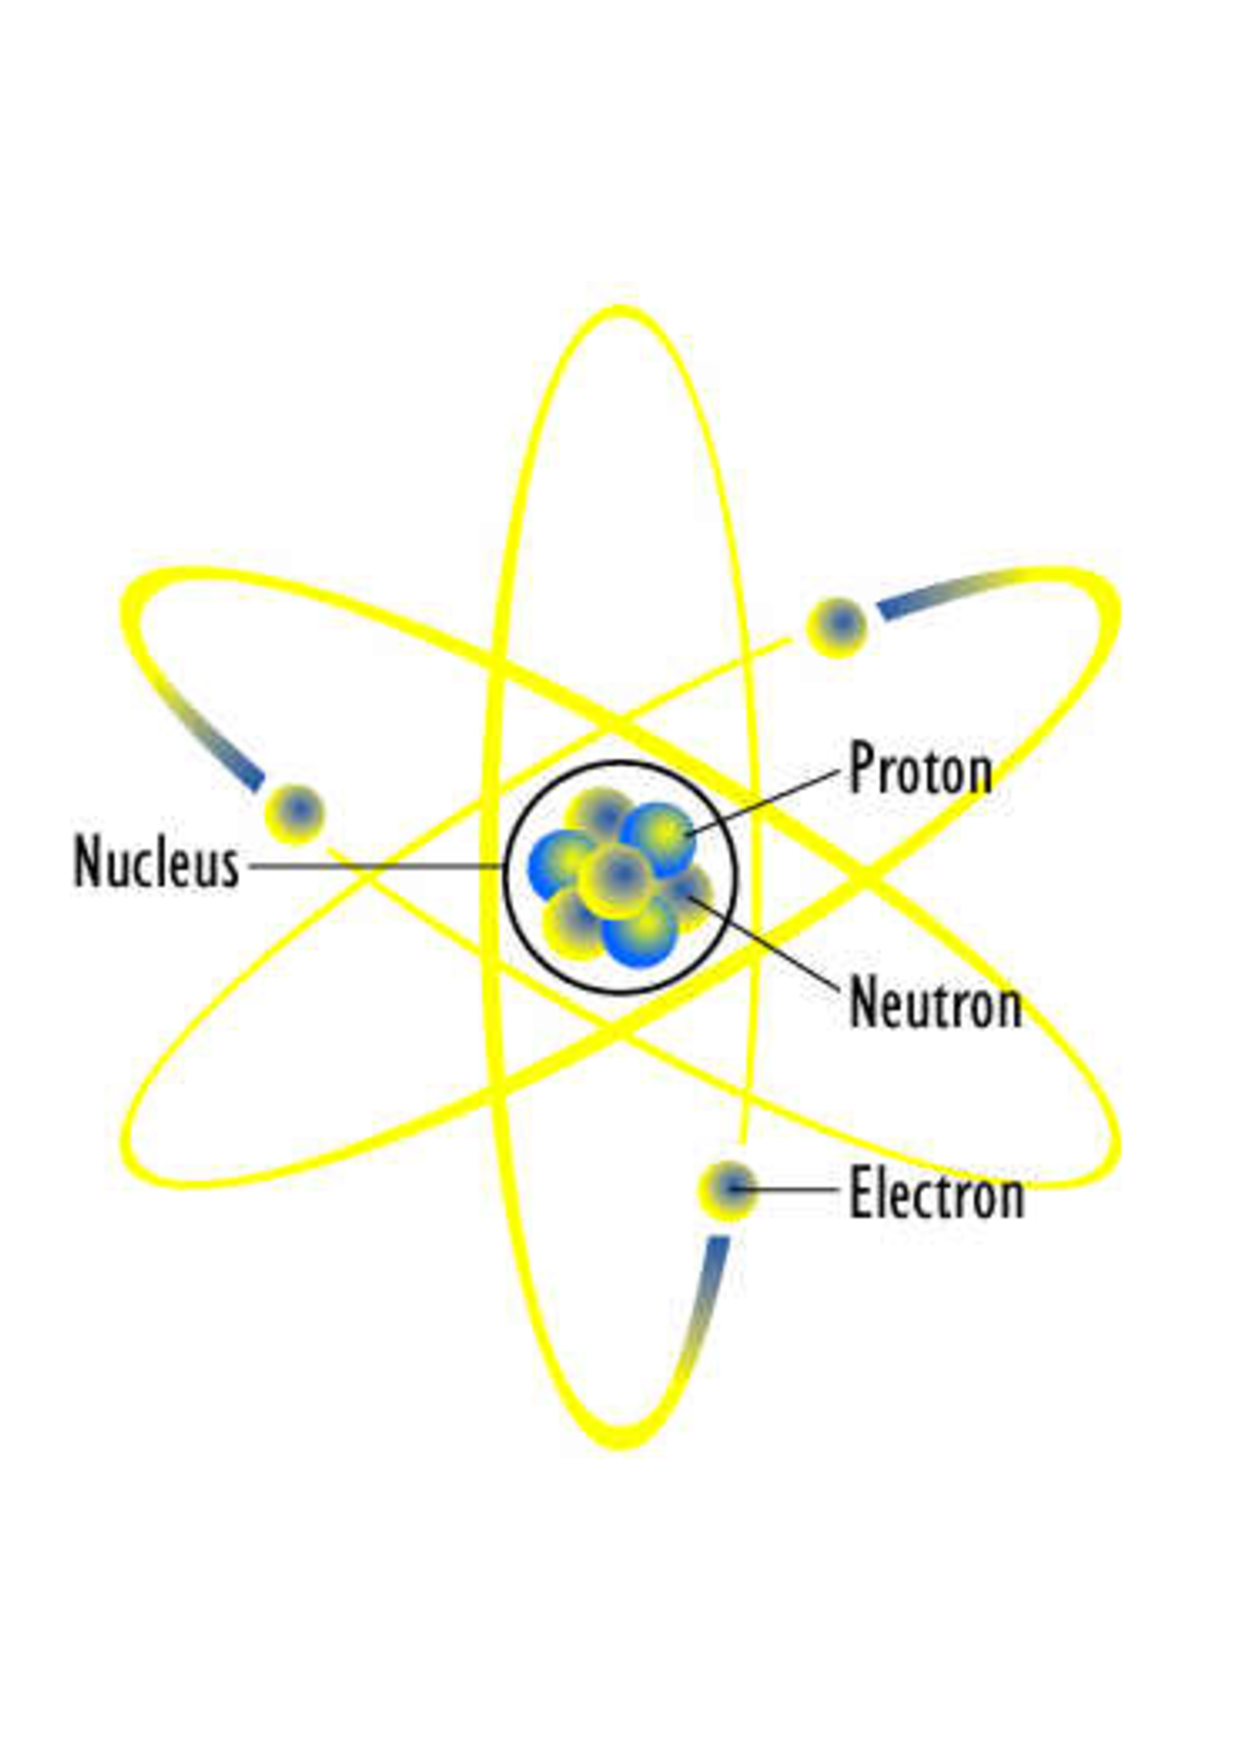
\includegraphics[scale=0.2]{Figures/bohr_1.pdf} & \centering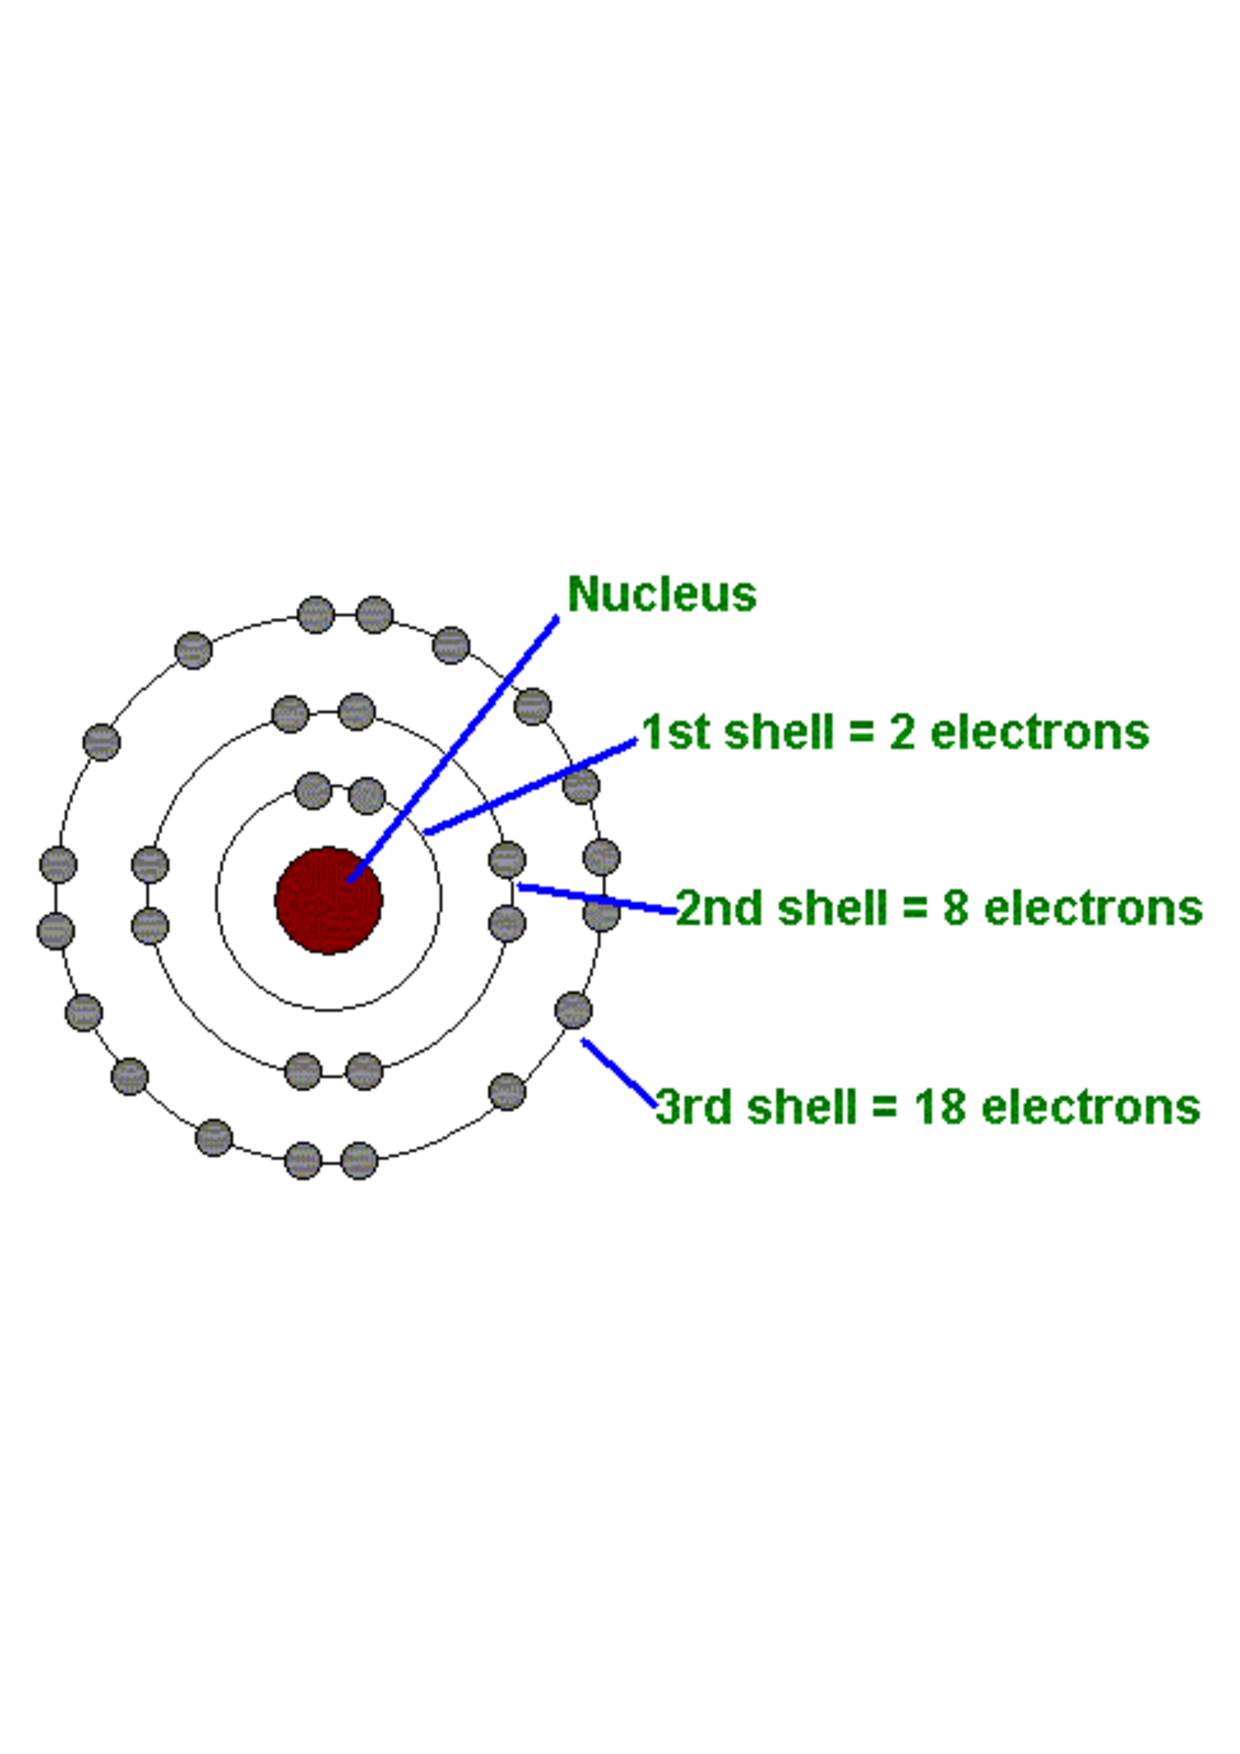
\includegraphics[scale=0.2]{Figures/bohr_2.pdf}
%%\end{tabular}
%%
%%\begin{block}{Energy levels}
%%Electrons further from the nucleus are at higher energy levels.
%%\end{block}
%%
%%\begin{exampleblock}{}
%%Electrons with the highest energy levels exist in the outermost shell of an atom and are relatively loosely bound to the atom. Electrons in this shell are called valence electrons.
%%\end{exampleblock}
%%\end{figure}
%%
%%
%%}
%%
%%\frame{
%%
%%\begin{block}{}
%%If an electron absorbs a photon with sufficient energy, it escapes from the atom and becomes a free electron. The atom becomes a positive ion.
%%\end{block}
%%
%%\begin{figure}
%%\centering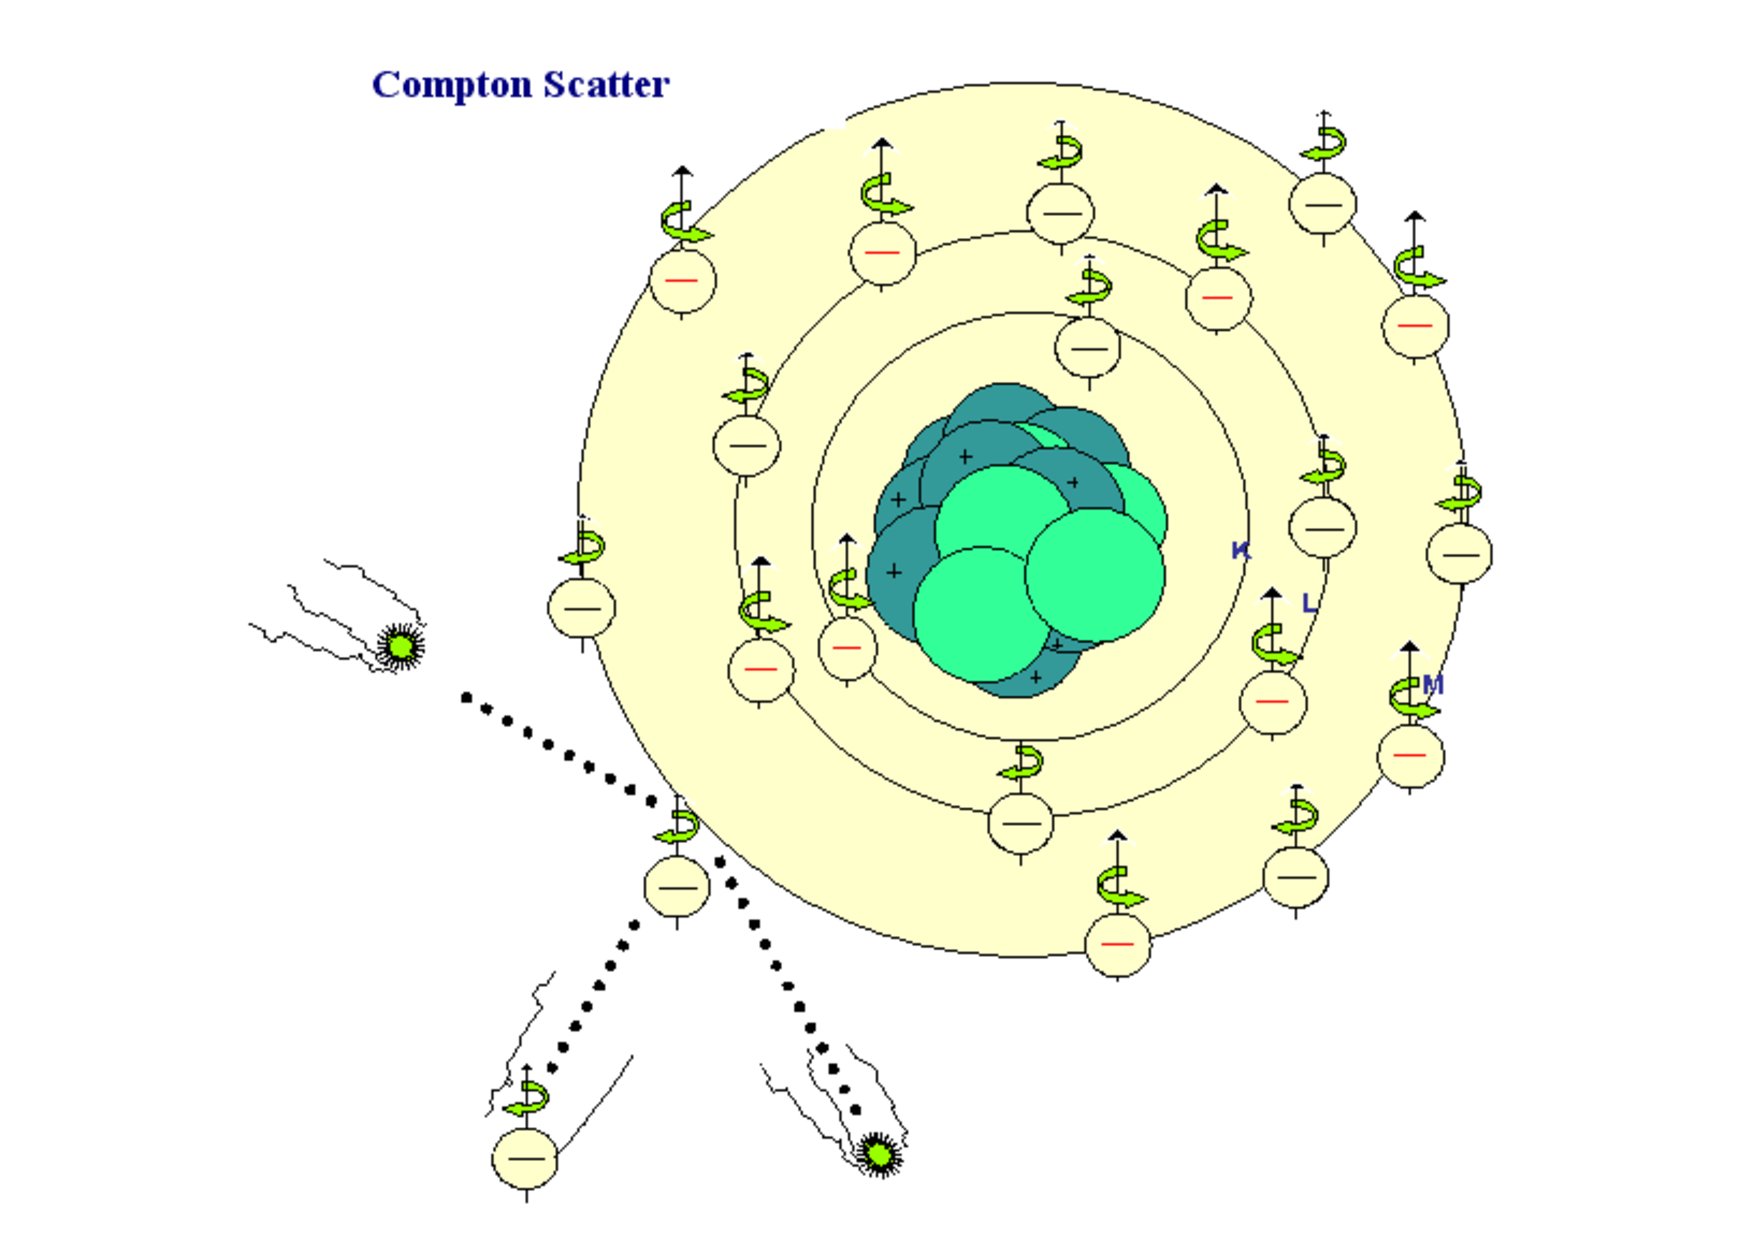
\includegraphics[scale=0.2]{Figures/free_elec.pdf}
%%\end{figure}
%%
%%
%%}
%%
%%\frame{
%%\frametitle{Conductors}
%%
%%\begin{itemize}
%%\item Materials that readily allow current. They have a large number of free electrons (cloud of free electrons). Metals are good conductors. Silver is the best conductor but the most widely used for wires is Copper (cheaper).
%%\item Semiconductor and insulator materials are characterized by decreasing conductivity properties. Namely, they have fewer free electrons in their structure. Insulators have no free electrons in their structure.
%%\end{itemize}
%%
%%}
%%
%%\frame{
%%\frametitle{Electrical Charge}
%%
%%\begin{itemize}
%%\item Property of matter: excess or deficiency of electrons. We symbolize the charge by $Q$.
%%\item The electron is the smallest particle that exhibits negative electrical charge.
%%\item Coulomb is the unit of charge. $Q_e=-1.6 10^{-19}$ C.
%%\item The charge of the proton is equal in magnitude to the electron charge, but with opposite sign.
%%\end{itemize}
%%
%%}
%%
%%\frame{
%%\frametitle{Electric field}
%%
%%\begin{itemize}
%%\item Materials with charges of opposite polarity are attracted to each other, and materials with charges of the same polarity are repelled.
%%\item Interpretation: a single or a set of elements with charge creates an electric field, which is the responsible to the movement of the charges.
%%\end{itemize}
%%
%%\begin{figure}
%%\centering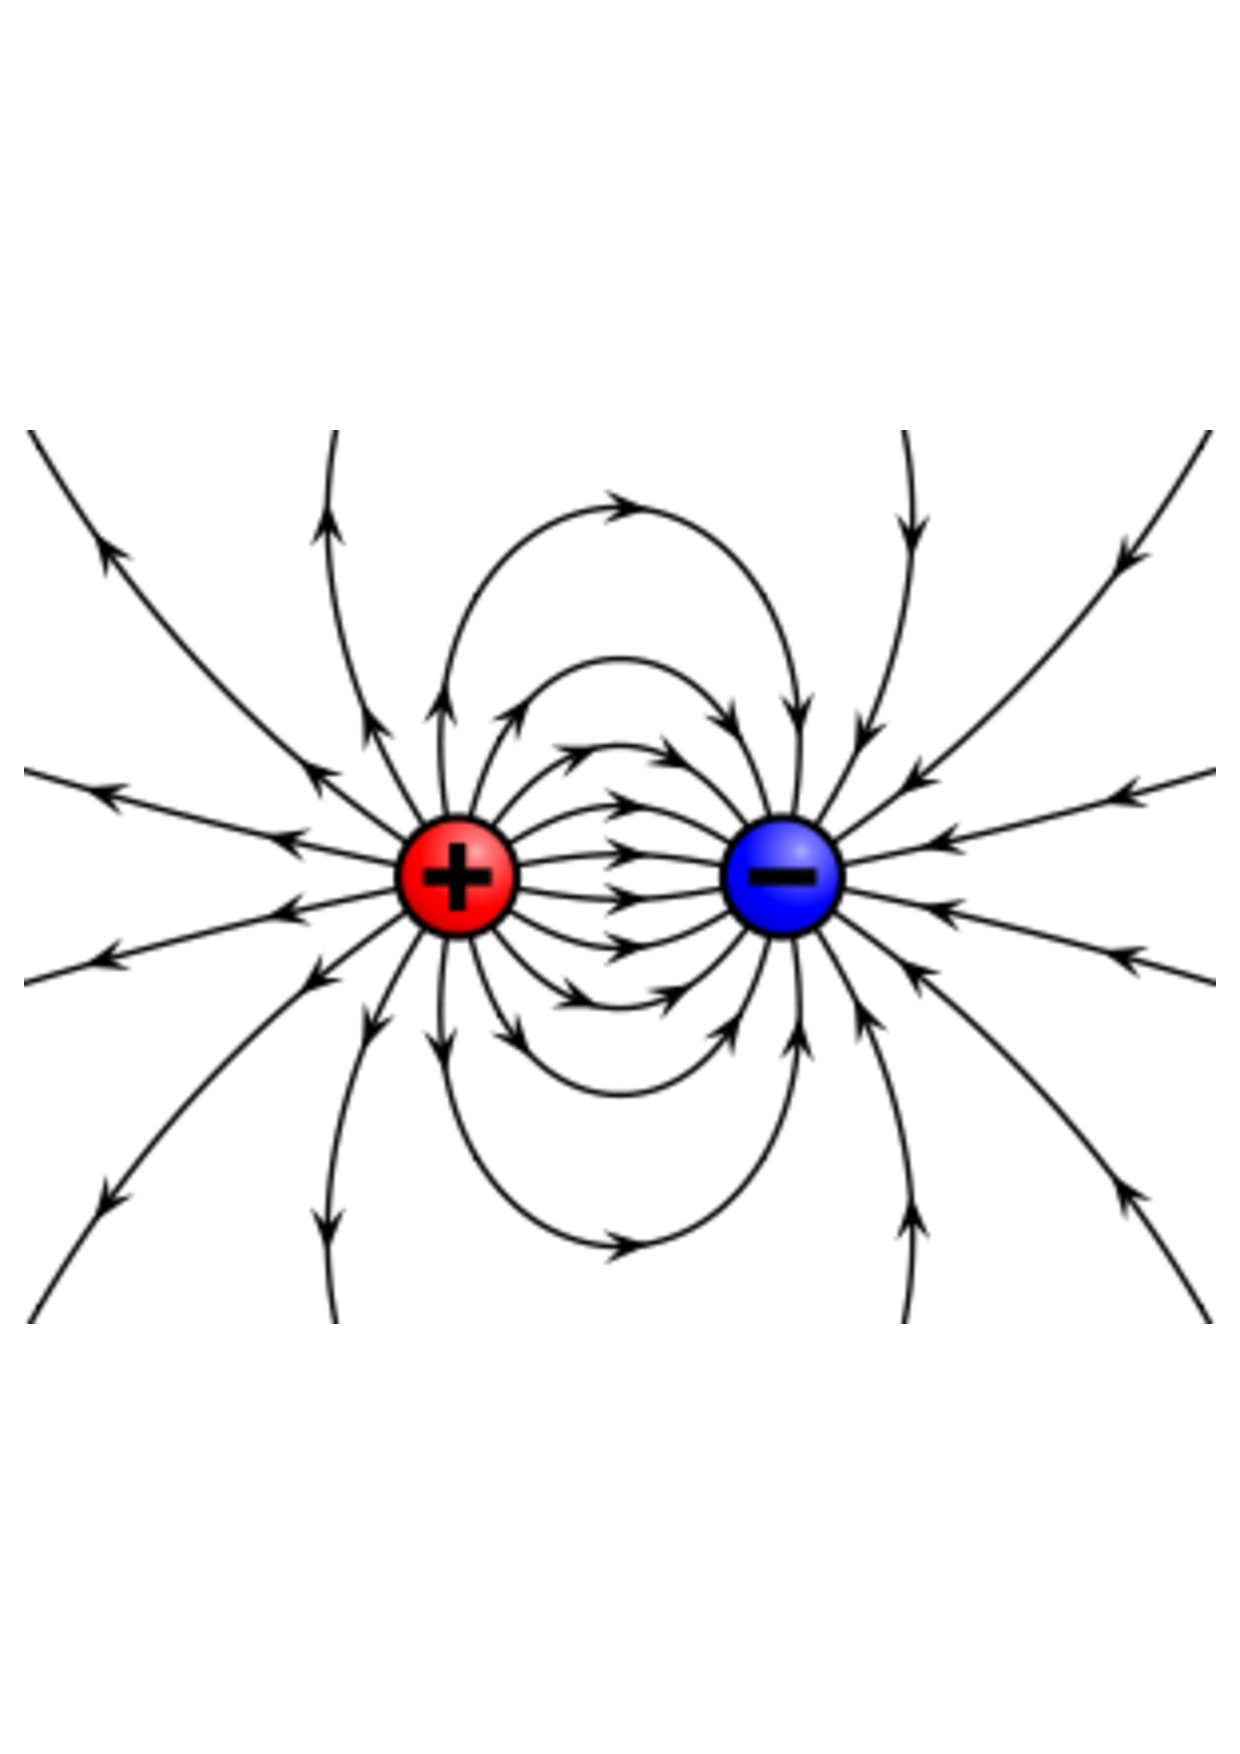
\includegraphics[scale=0.2]{Figures/efield.pdf}
%%\end{figure}
%%
%%\begin{block}{}
%%Any charge placed in a point A of an electric field has a given energy $W_A$ (Joules). Movinge the charge between point A and point B requires an energy $W_B-W_A$.
%%\end{block}
%%
%%
%%
%%}
%
%\frame{
%\begin{block}{Voltage or potential}
%Energy per unit charge:
%\begin{align}\nonumber 
%V=\frac{\partial W}{\partial Q}\qquad \text{volts (V)}
%\end{align}
%One volt is the potential difference between two points when one joule of energy is used to move one coulomb of positive charge from one point to the other.  
%\end{block}
%
%\begin{columns}
%\begin{column}{0.5\textwidth}
%\begin{figure}
%\centering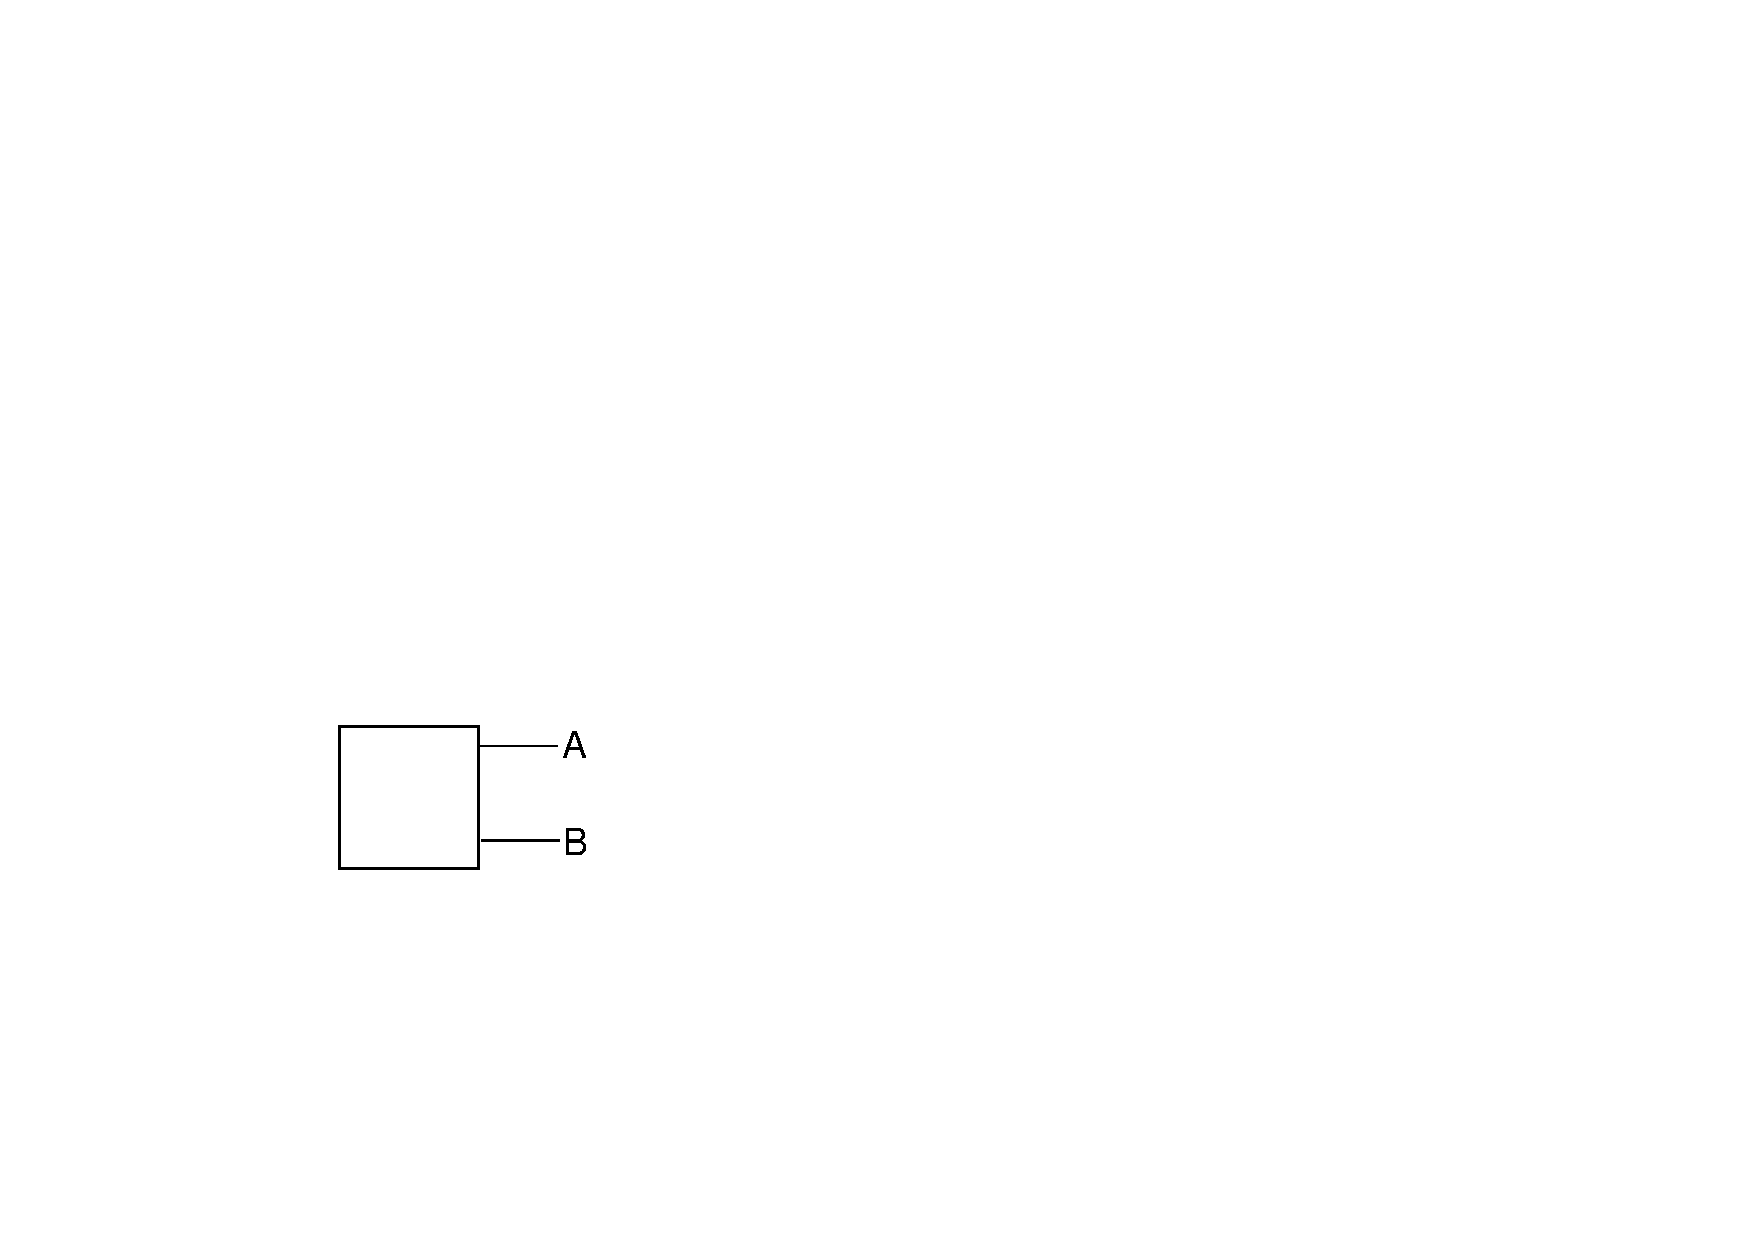
\includegraphics[scale=0.8]{Figures/potAB.pdf}
%\end{figure}
%\end{column}
%\begin{column}{0.5\textwidth}
%\begin{itemize}
%\item $V_{AB}=V_A-V_B>0 \rightarrow $ when a \underline{positive charge} goes from A to B it losses energy. 
%\item $V_{AB}=V_A-V_B<0 \rightarrow $ when a \underline{positive charge}  goes from A to B it wins energy. 
%\end{itemize}
%\end{column}
%\end{columns}
%
%}
%
%
%\frame{
%\frametitle{The ideal Voltage Source}
%
%\begin{center}
%\begin{circuitikz} \draw 
%  (0,0) to[V] (0,2)
%  to[short,o-*](2,2)
%  (0,0) to[short,o-*](2,0)
%  (3,2) node[anchor=east] {A}
%  (3,0) node[anchor=east] {B}
%  (-0.5,1) node[anchor=east] {$V_s$}
%   (6,1) node[anchor=east] {$V_s=V_A-V_B$};
%%       to[R=1<\ohm>] (2,2) 
%%        to[C=1<\farad>] (2,0) -- (0,0);
%\end{circuitikz}
%\end{center}
%
%\begin{block}{}
%An ideal voltage source can provide a constant voltage for any current required by a circuit.
%\end{block}
%}
%
%\frame{
%\frametitle{Electrical current in a conductor/semiconductor}
%
%\begin{itemize}
%\item Under normal conditions the movement of the electrons is truly random, meaning they are moving in all directions by the same amount.
%\item If a voltage is placed across a conductive material, it causes the free electrons to move in a single direction. 
%\item We define the electrical current as the rate of charge flow past a given point in an electric circuit:
%\begin{align}\nonumber
%I(t)=\frac{\partial Q(t)}{\partial t} \qquad \text{Amperes (A)}
%\end{align}
%
%
%\end{itemize}
%
%\begin{columns}
%\begin{column}{0.5\textwidth}
%\begin{figure}
%\centering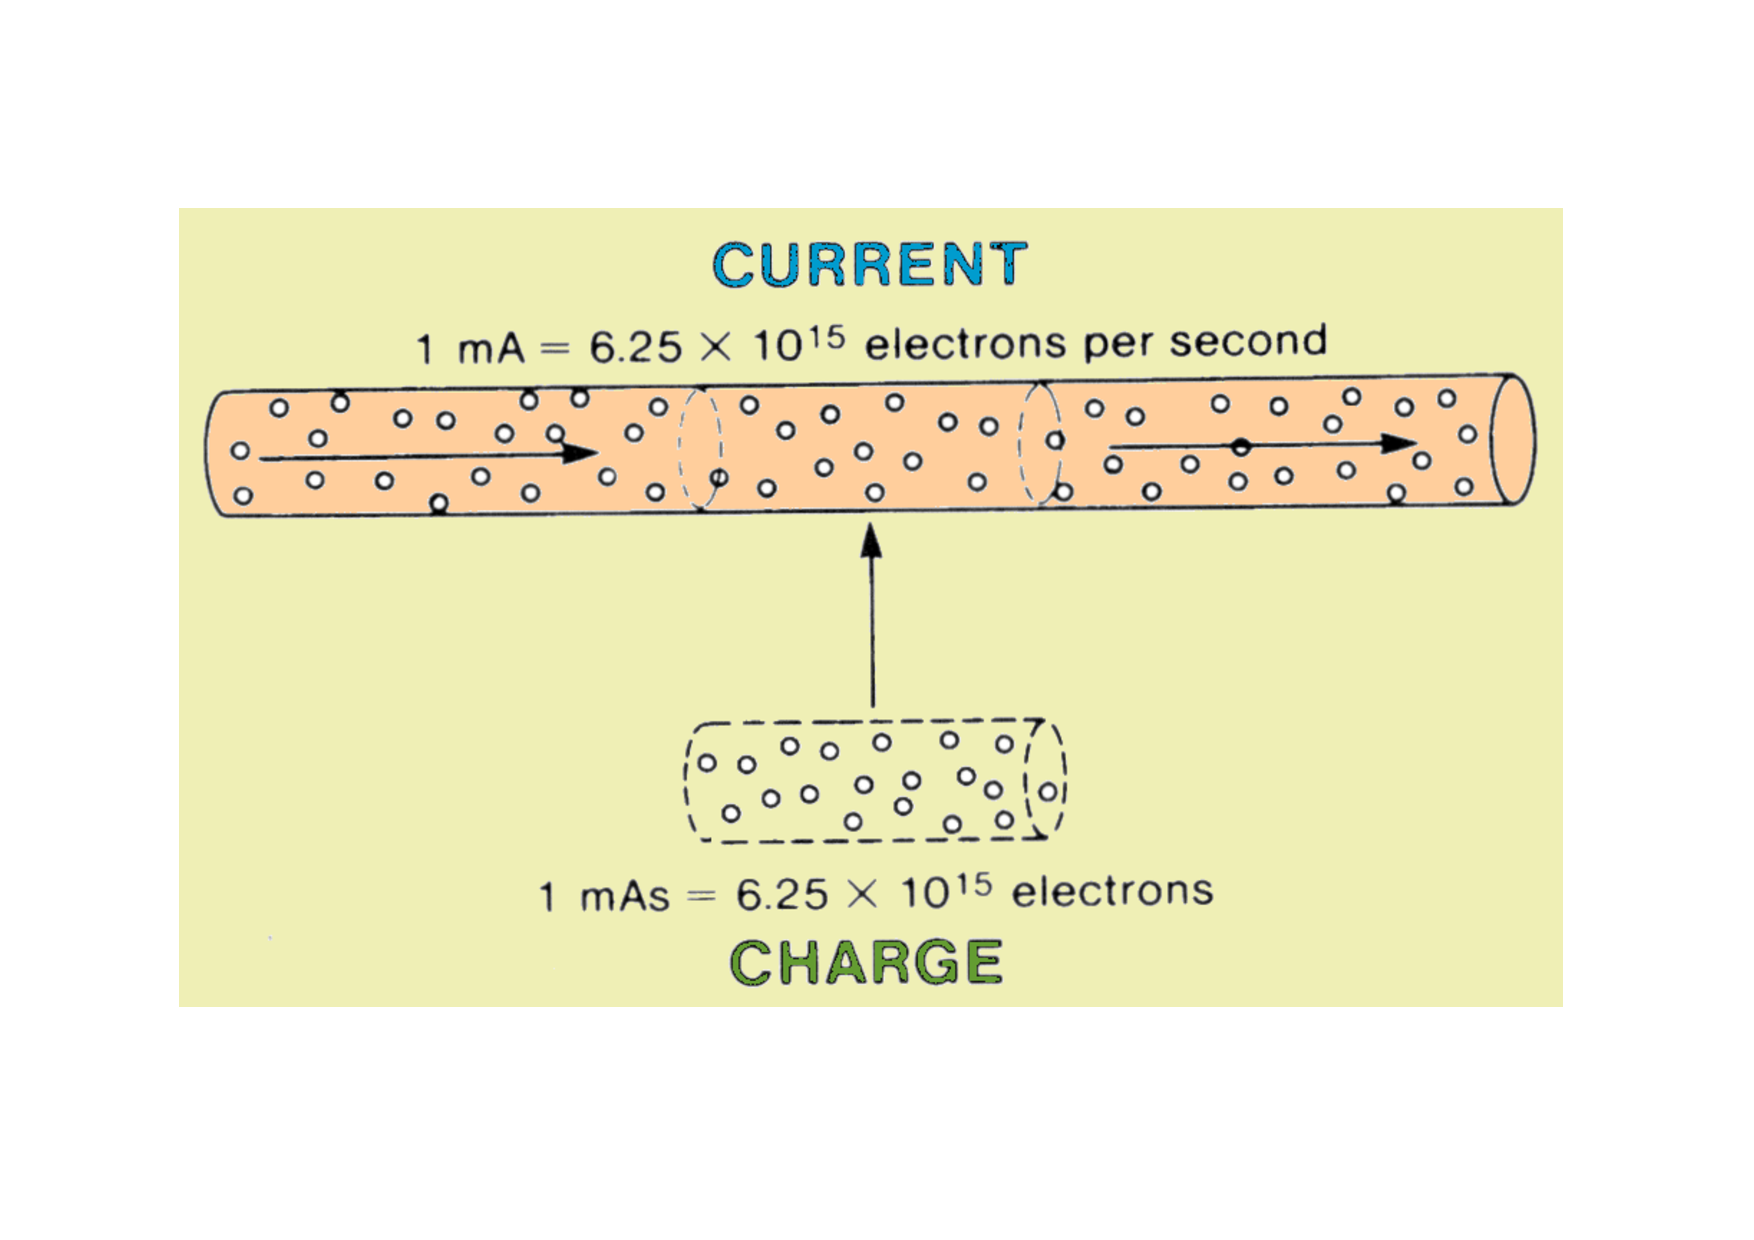
\includegraphics[scale=0.25]{Figures/current.pdf}
%\end{figure}
%\end{column}
%\begin{column}{0.5\textwidth}
%\begin{block}{}
%One ampere is the amount of current that exists when a number of electrons having a total charge of one coulomb move trough a given cross-sectional area in one second.
%\end{block}
%\end{column}
%\end{columns}
%
%}
%
%\frame{
%\frametitle{Conventional current flow}
%
%\begin{itemize}
%\item We consider the current as a flow of positive charges.
%\item Just a criterion, the real flow of charge is composed by electrons moving in the opposite direction. 
%\item Using our convention, the current goes from the point of higher voltage to the point of lower voltage. 
%\end{itemize}
% 
%\begin{figure}
%\centering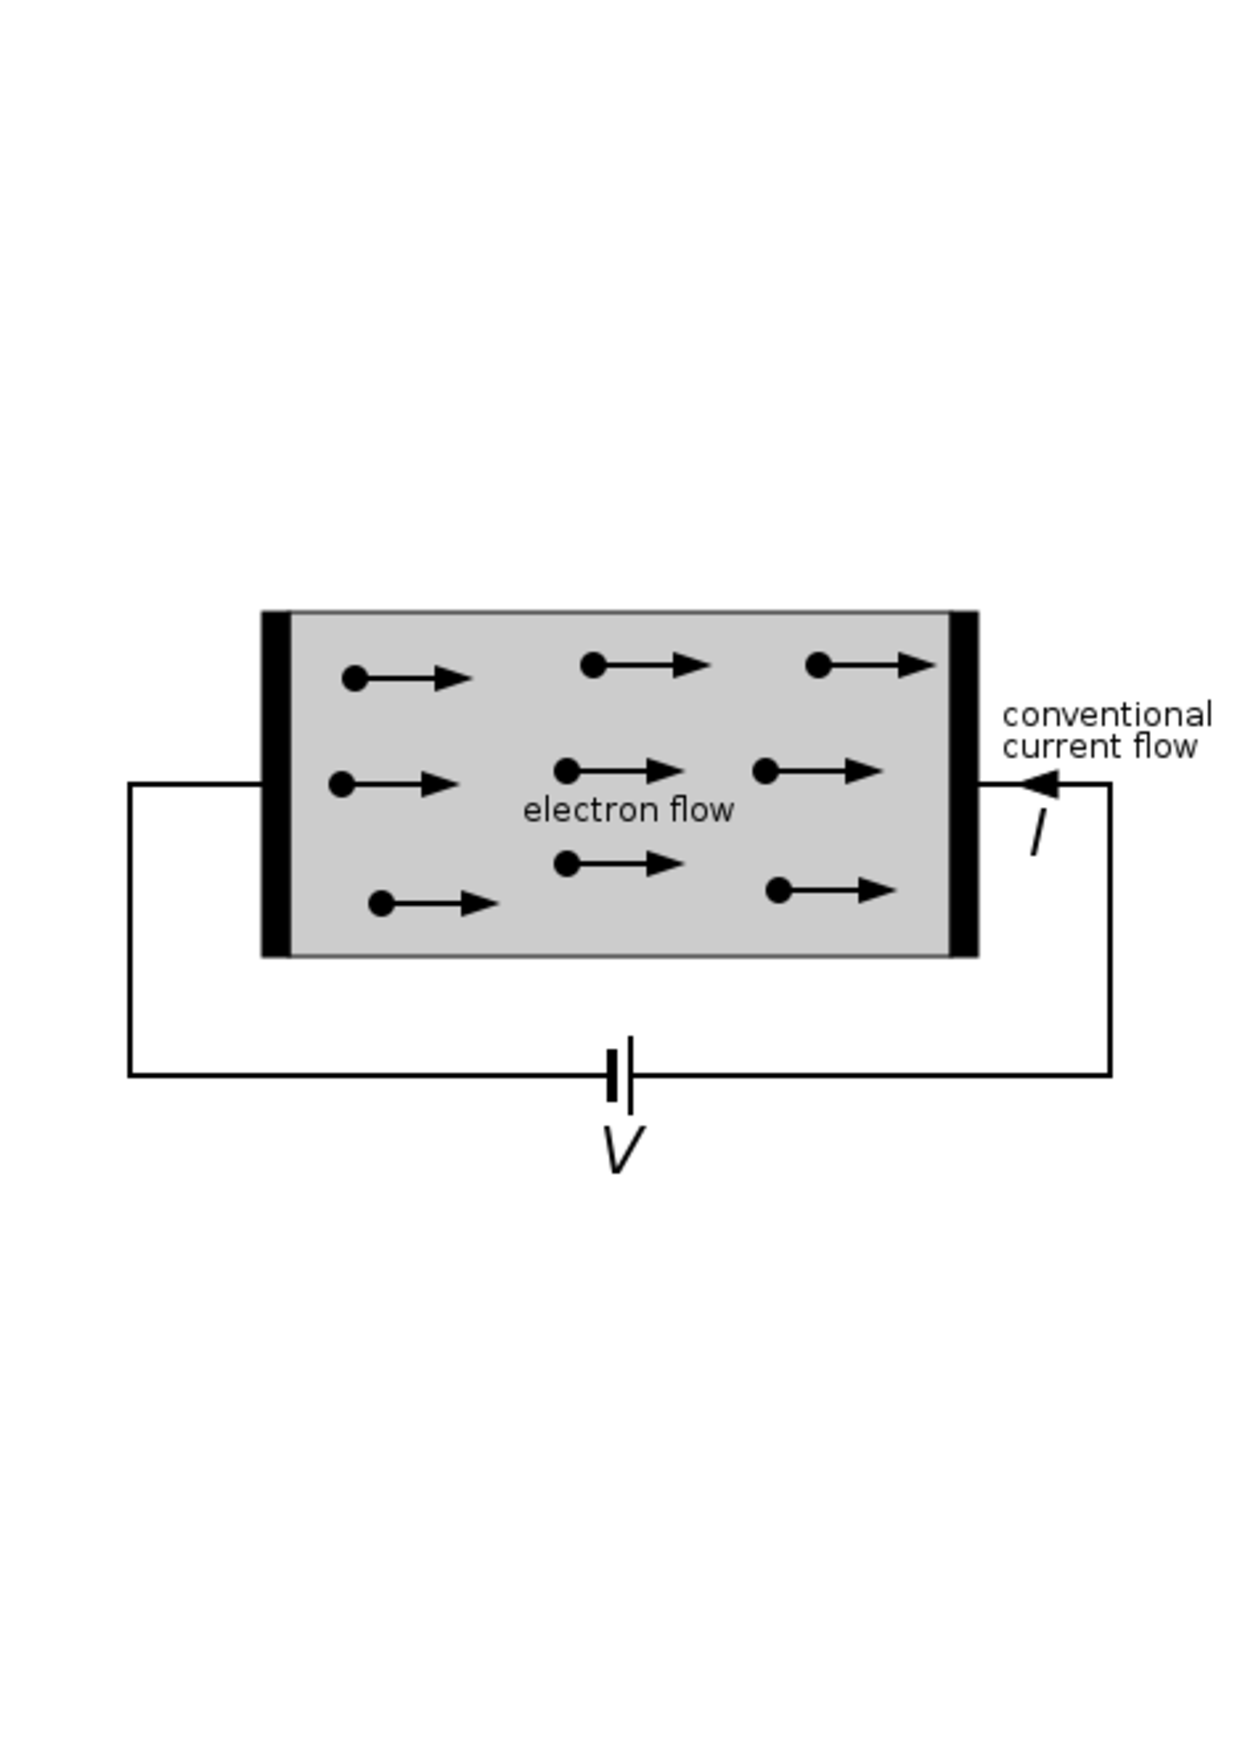
\includegraphics[scale=0.25]{Figures/conv_current.pdf}
%\end{figure}
%
%}
%
%
%\frame{
%\frametitle{Electric Power}
%
%\begin{itemize}
%\item Assume a voltage $V(t)$ between both extremes of a two-terminal device in an electric circuit and a given current $I(t)$ moving throughout it.
%\item Electric power $P(t)$ is the amount of electric energy $W(t)$ used per unit time:
%\begin{align}\nonumber
%P(t)=\frac{\partial W(t)}{\partial t}=\frac{\partial W(t)}{\partial Q(t)}\frac{\partial Q(t)}{\partial t}=V(t)I(t) \qquad \text{Watts (W)}
%\end{align} 
%\end{itemize}
%
%
%\begin{columns}
%\begin{column}{0.5\textwidth}
%\begin{figure}
%\centering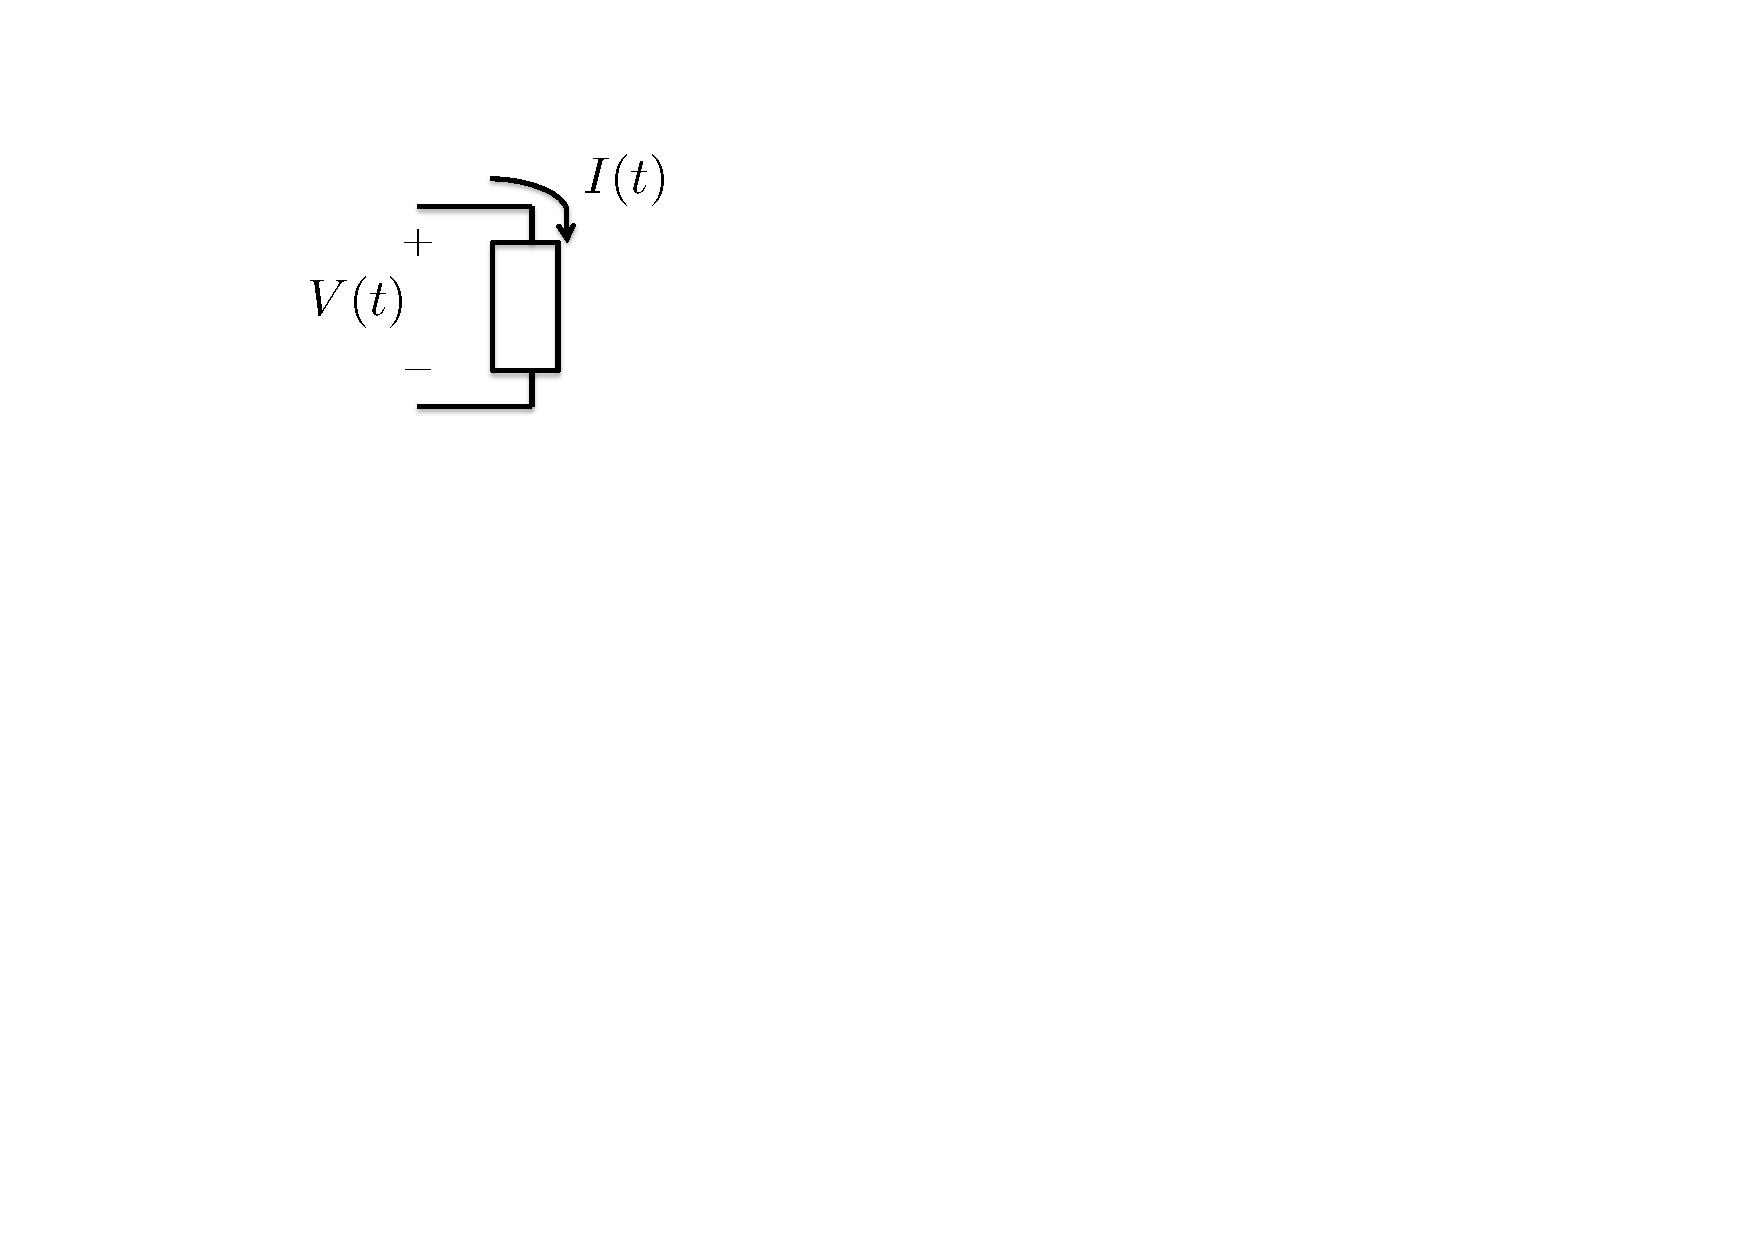
\includegraphics[scale=0.5]{Figures/power_1.pdf}
%\end{figure}
%\end{column}
%\begin{column}{0.5\textwidth}
%\begin{itemize}
%\item The charges flow from a point of higher potential to a point of lower potential $\Rightarrow$ They are losing energy.
%\item[$\Rightarrow$] $P(t)>0$: the device is consuming power.
%\end{itemize}
%\end{column}
%\end{columns}
%
%} 
%
%\frame{
%\frametitle{Electric Power}
%\begin{figure}
%\centering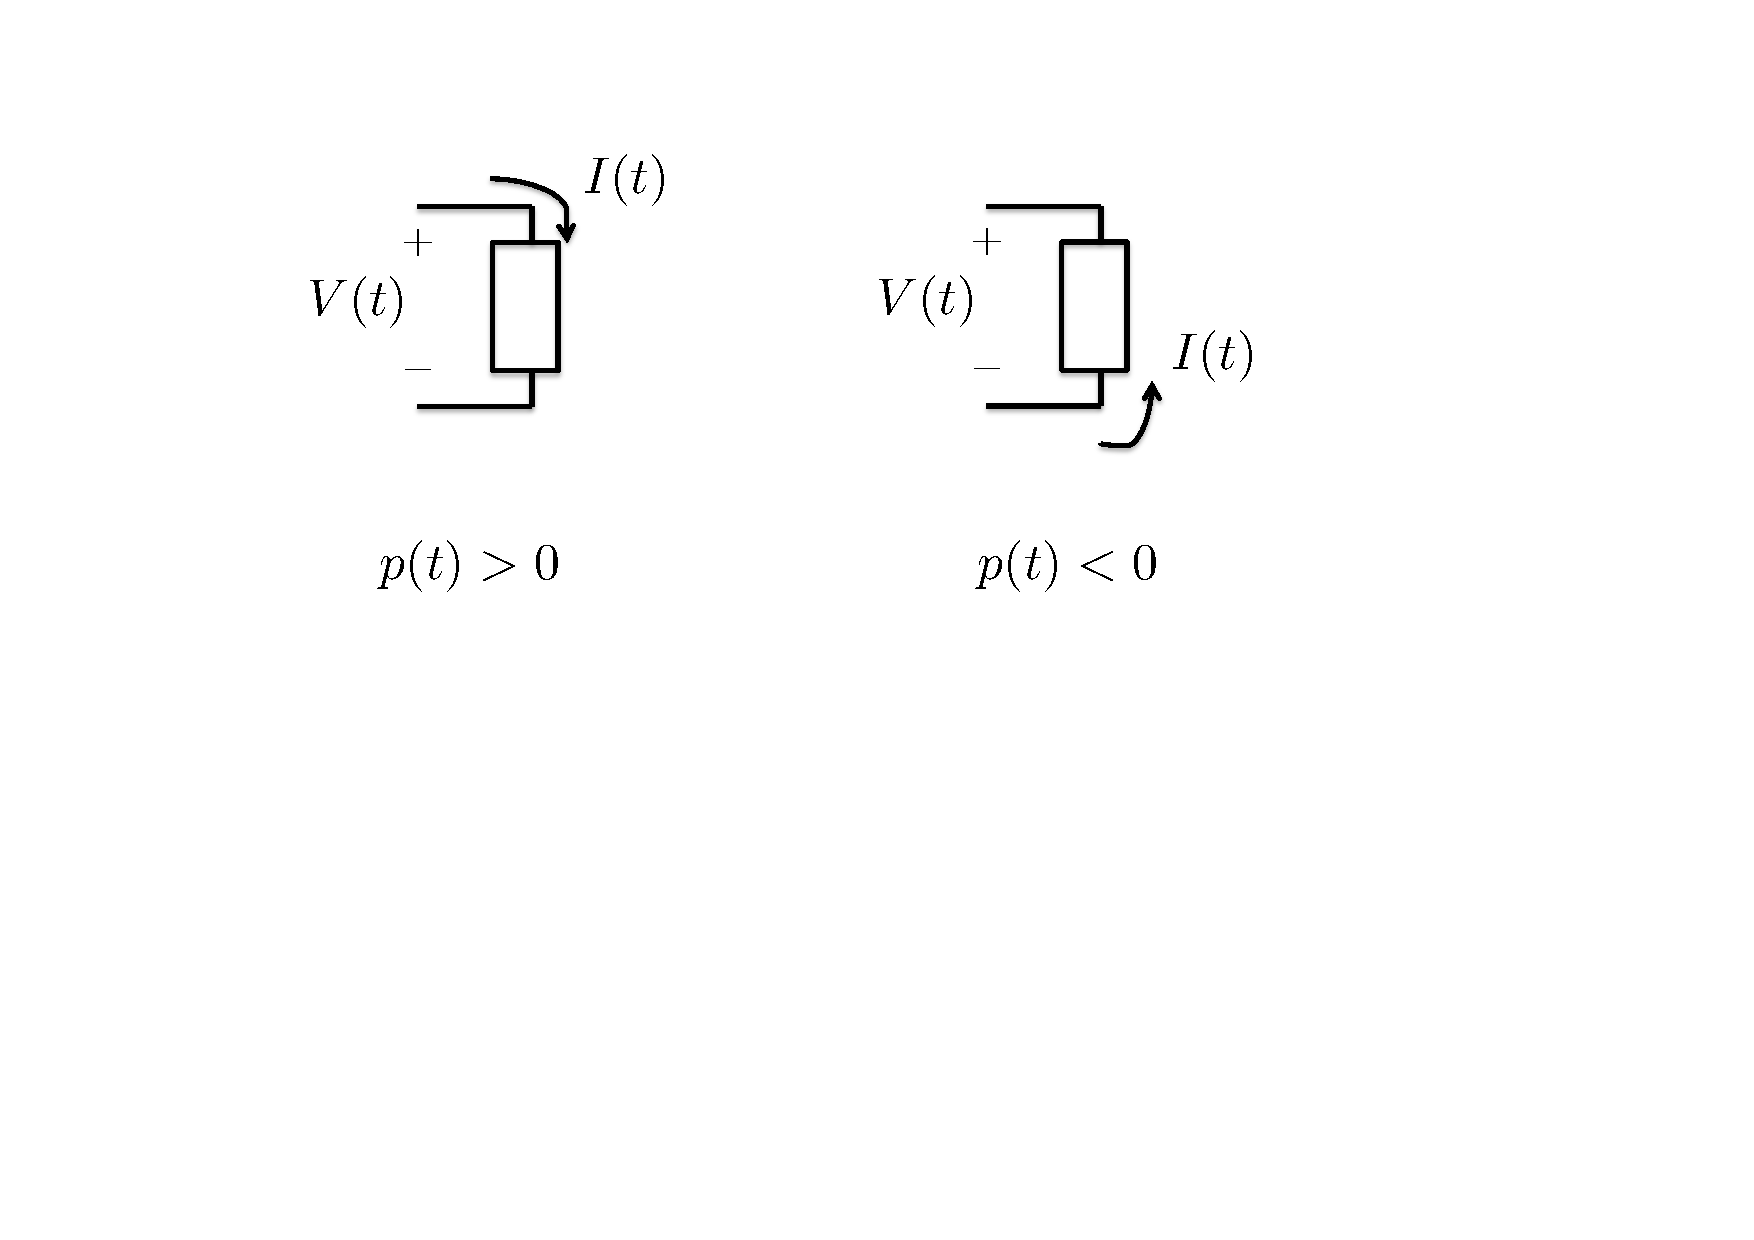
\includegraphics[scale=0.5]{Figures/power_2.pdf}
%\end{figure}
%
%In the second case, the current goes from a point of lower voltage to a point of higher voltage.  The charges win energy $\Rightarrow$ the device is generating power.
%
%\begin{exampleblock}{}
%Any device that generates power is said to be active (e.g. a voltage source) and otherwise passive (a resistor).
%\end{exampleblock}
%
%%\begin{columns}
%%\begin{column}{0.5\textwidth}
%%\begin{center}
%%\begin{circuitikz} \draw 
%%  (0,2) to[short](2,2)
%%  to[R](2,0)
%%  to[short](0,0)
%%  (0,1)node[anchor=east] {$V(t)$};
%%%  (0,0) to[V] (0,2)
%%%  to[short,o-*](2,2)
%%%  (0,0) to[short,o-*](2,0)
%%%  (3,2) node[anchor=east] {A}
%%%  (3,0) node[anchor=east] {B}
%%%  (-0.5,1) node[anchor=east] {$V_s$}
%%%   (6,1) node[anchor=east] {$V_s=V_A-V_B$};
%%%       to[R=1<\ohm>] (2,2) 
%%%        to[C=1<\farad>] (2,0) -- (0,0);
%%\end{circuitikz}
%%\end{center}
%%\end{column}
%%\begin{column}{0.5\textwidth}
%%\begin{circuitikz} \draw 
%%  (2,0) to[V](2,2)
%%  to[short](0,2)
%%  (0,0) to[short](2,0);
%%%  (0,0) to[V] (0,2)
%%%  to[short,o-*](2,2)
%%%  (0,0) to[short,o-*](2,0)
%%%  (3,2) node[anchor=east] {A}
%%%  (3,0) node[anchor=east] {B}
%%%  (-0.5,1) node[anchor=east] {$V_s$}
%%%   (6,1) node[anchor=east] {$V_s=V_A-V_B$};
%%%       to[R=1<\ohm>] (2,2) 
%%%        to[C=1<\farad>] (2,0) -- (0,0);
%%\end{circuitikz}
%%\end{column}
%%\end{columns}
%
%}
%
%\section{Elements of a resistive circuit}
%
%\frame{
%\frametitle{Ideal Voltage source}
%
%\begin{center}
%\begin{circuitikz} \draw 
%  (0,0) to[V] (0,2)
%  to[short,o-*](2,2)
%  (0,0) to[short,o-*](2,0)
%  (3,2) node[anchor=east] {A}
%  (3,0) node[anchor=east] {B}
%  (-0.5,1) node[anchor=east] {$V_s$}
%   (6,1) node[anchor=east] {$V_s=V_A-V_B$};
%%       to[R=1<\ohm>] (2,2) 
%%        to[C=1<\farad>] (2,0) -- (0,0);
%\end{circuitikz}
%\end{center}
%
%\begin{block}{}
%An ideal voltage source can provide a constant voltage for any current required by a circuit.
%\end{block}
%
%}
%
%\frame{
%\frametitle{Voltage sources in series}
%
%\begin{block}{}
%When two or more voltage sources are in series, the total voltage is equal to the algebraic sum of the individual source voltages.
%\end{block}
%
%\begin{columns}
%\begin{column}{0.5\textwidth}
%\begin{center}
%\begin{circuitikz} \draw 
%  (0,0) to[V] (0,2)
%  to[V](0,4)
%  to[V](0,6)
%  to[short,o-*](2,6)
%  (0,0) to[short,o-*] (2,0)
%  (2.5,6) node[anchor=east] {$A$}
%  (2.5,0) node[anchor=east] {$B$}
%  (5,3) node[anchor=east] { $V_A-V_B=V_1+V_2+V_3$}
%  (-0.5,1) node[anchor=east] {$V_1$}
%  (-0.5,3) node[anchor=east] {$V_2$}
%  (-0.5,5) node[anchor=east] {$V_1$};
%\end{circuitikz}
%\end{center}
%\end{column}
%\begin{column}{0.5\textwidth}
%\vspace{0.3cm}
%\begin{circuitikz} \draw 
%  (0,0) to[V] (0,2)
%  (0,4) to[V] (0,2)
%  (0,4) to[V] (0,6)
%  to[short,o-*](2,6)
%  (0,0) to[short,o-*] (2,0)
%  (2.5,6) node[anchor=east] {$A$}
%  (2.5,0) node[anchor=east] {$B$}
%  (5,3) node[anchor=east] { $V_A-V_B=V_1-V_2+V_3$}
%  (-0.5,1) node[anchor=east] {$V_1$}
%  (-0.5,3) node[anchor=east] {$V_2$}
%  (-0.5,5) node[anchor=east] {$V_1$};
%\end{circuitikz}
%\end{column}
%\end{columns}
%
%}
%
%
%\frame{
%\frametitle{Ideal current source}
%
%\begin{center}
%\begin{circuitikz} \draw 
%  (0,0) to[I] (0,2)
%  to[short,o-*](2,2)
%  (0,0) to[short,o-*](2,0)
%  (-0.5,1) node[anchor=east] {$I_s$};
%%       to[R=1<\ohm>] (2,2) 
%%        to[C=1<\farad>] (2,0) -- (0,0);
%\end{circuitikz}
%\end{center}
%
%\begin{block}{}
%An ideal voltage source can provide a constant current for any voltage required by a circuit.
%\end{block}
%
%}
%
%
%\frame{
%\frametitle{Current sources in parallel}
%
%\begin{block}{}
%The total current produced by current sources in parallel is equal to the algebraic sum of the individual current sources.
%\end{block}
%
%\begin{center}
%\begin{circuitikz} \draw 
%  (0,0) to[I] (0,2)
%  to[short,o-*](6,2)
%  (0,0) to[short,o-*](6,0)
%  (-0.5,1) node[anchor=east] {$I_1$}
%  (2,0) to[I] (2,2)
%  (1.5,1) node[anchor=east] {$I_2$}
%  (4,0) to[I] (4,2)
%  (3.5,1) node[anchor=east] {$I_3$}
%  (6,2) to[R] (6,0);
%\end{circuitikz}
%\end{center}
%
%\begin{center}
%\begin{circuitikz} \draw 
%  (0,0) to[I] (0,2)
%  to[short,o-*](2,2)
%  to [R] (2,0)
%  (-1,1) node[anchor=east] {$I_1+I_2+I_3$}
%  (0,0) to[short,o-*](2,0);
%\end{circuitikz}
%\end{center}
%}
%
%\frame{
%\frametitle{Branches, Loops and nodes}
%
%\begin{itemize}
%\item Branch: any element of two terminals (wires do not count).
%\item Loop: any set of branches that form a closed loop.
%\item Minimal loop: any loop that does not contain another loop.
%\item Node: a node is any point or junction in a circuit where two or more components are connected.
%\end{itemize}
%
%\begin{figure}
%\centering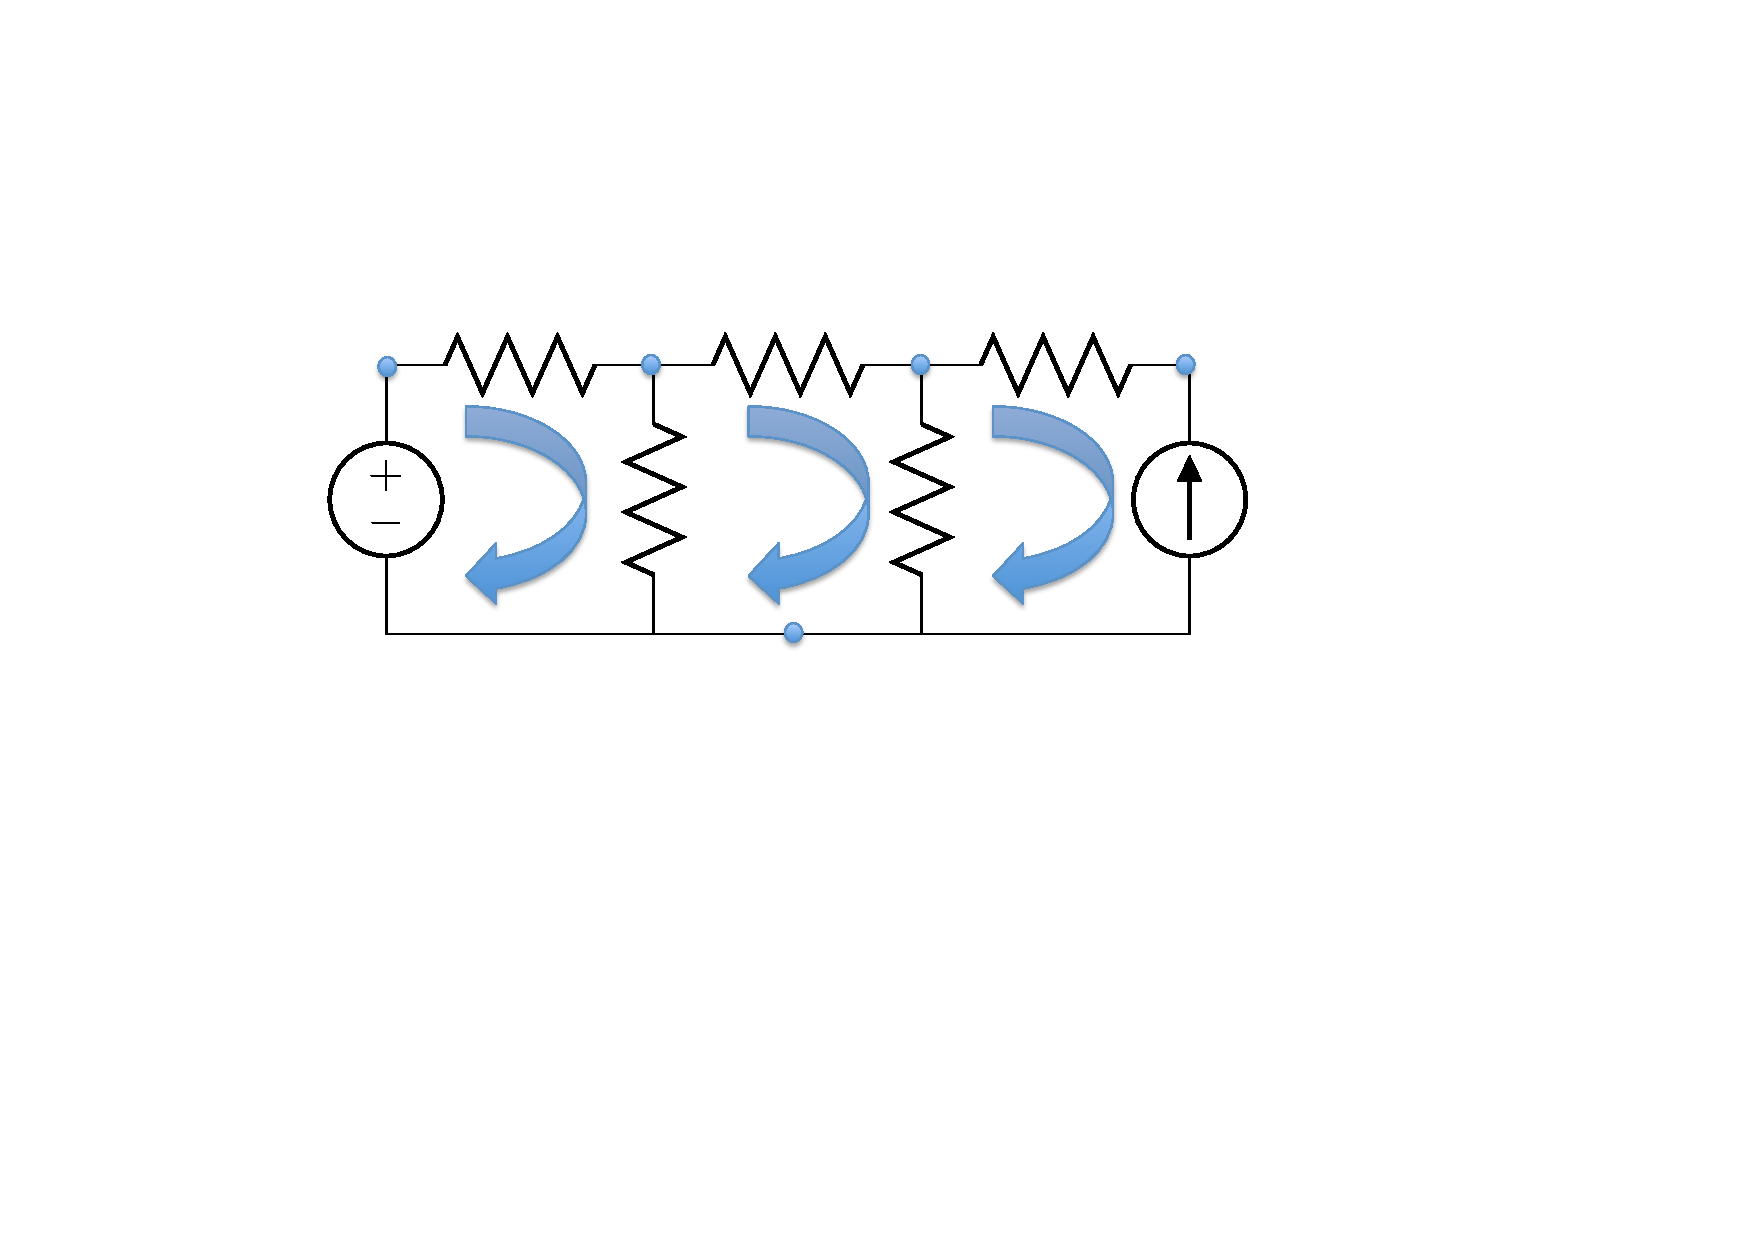
\includegraphics[scale=0.5]{Figures/loops_nodes.pdf}
%\caption{7 devices or branches, 3 minimal loops and 5 nodes.}
%\end{figure}
%}
%
%\section{Kirchhoff's laws}
%
%\frame{
%\frametitle{Kirchhoff's current law}
%
%\begin{block}{}
%The sum of the currents into a node (total current in) is equal to the sum of the currents out of a node (total current out).
%\end{block}
%
%
%\begin{center}
%\begin{circuitikz} \draw 
%  (0,0) to[V=$V_s$] (0,2)
%  to[short,-*,i=$I_s$](1,2)
%  to[short](1,1)
%  to[short](1,3)
%  (1,2) to[R=$R_2$,i=$I_2$](3,2)
%  to[short,*-,i=$I_s$](4,2)
%  (1,1) to[R=$R_1$,i=$I_1$](3,1)
%    to[short](3,2)
%  (1,3) to[R=$R_3$,i=$I_3$](3,3)
%    to[short](3,2)
%   (4,2) to[short](4,0)
%    to[short](0,0)
%   (1.05,1.80) node[anchor=east] {A}
%   (3.45,1.80) node[anchor=east] {B};
%\end{circuitikz}
%\end{center}
%
%\begin{columns}
%\begin{column}{0.5\textwidth}
%\textbf{In node A}
%\begin{align}\nonumber
%\underbrace{I_s}_{\text{Current in}}=\underbrace{I_1+I_2+I_3}_{\text{Current out}}
%\end{align}
%\end{column}
%\begin{column}{0.5\textwidth}
%\textbf{In node B}
%\begin{align}\nonumber
%\underbrace{I_1+I_2+I_3}_{\text{Current in}}=\underbrace{I_s}_{\text{Current out}}
%\end{align}
%\end{column}
%\end{columns}
%
%
%
%}
%
%
%\frame{
%\frametitle{Kirchhoff's voltage law}
%\begin{block}{}
%The sum of all the voltage drops around a singled closed path in a circuit is equal to the total source voltage in that loop.
%\end{block}
%
%\begin{columns}
%\begin{column}{0.5\textwidth}
%\begin{center}
%\begin{circuitikz} \draw 
%  (0,-1) to[V=$V_s$,i=$I_s$] (0,5)
%  to[short](2,5)
%  to[short](2,4.9)
%  %[european voltages]
%  (2,4.89) to[R=$R_1$,v=$V_1$](2,3)
%  to[R=$R_2$,v=$V_2$](2,1)
%  to[R=$R_3$,v=$V_3$](2,-1)
%  to[short](0,-1);
%\end{circuitikz}
%\end{center}
%\end{column}
%\begin{column}{0.5\textwidth}
%\begin{align}\nonumber
%V_s=V_1+V_2+V_3
%\end{align}
%\begin{block}{}
%Basic tools to analyze resistive circuits: Kirchhoff's laws + Ohm's law.
%\end{block}
%\end{column}
%\end{columns}
%
%}
%
%\frame{
%\frametitle{Kirchhoff's voltage law}
%
%Another way, and usually more useful, way to express Kirchhoff's voltage law is as follows:
%\begin{block}{}
%The algebraic sum of all voltage drops around a single closed path is zero. 
%\end{block}
%
%\begin{columns}
%\begin{column}{0.5\textwidth}
%\begin{center}
%\begin{circuitikz} \draw 
%  (0,-1) to[V=$V_s$,i=$I_s$] (0,5)
%  to[short](2,5)
%  to[short](2,4.9)
%  %[european voltages]
%  (2,4.89) to[R=$R_1$,v=$V_1$](2,3)
%  to[R=$R_2$,v=$V_2$](2,1)
%  to[R=$R_3$,v=$V_3$](2,-1)
%  to[short](0,-1);
%\end{circuitikz}
%\end{center}
%\end{column}
%\begin{column}{0.5\textwidth}
%We follow the current and algebraically sum the voltage drops. A voltage source represents a negative drop. 
%\begin{align}\nonumber
%V_1+V_2+V_3\color{red}{-V_s}=\color{black}{0}
%\end{align}
%\end{column}
%\end{columns}
%
%}
%
%
%
%
%\section{Loop current method and Node voltage method}
%
%\frame{
%\frametitle{Simultaneous equations in Circuits analysis}
%
%\begin{itemize}
%\item Using Kirchhoff's voltage and current laws we derive a set of linear equations where the voltages/currents of interests are the unknowns. Then, we make use of linear algebra to solve the system of equations. 
%\item We present two methods: the loop current method and the node voltage method.
%\end{itemize}
%
%\begin{alertblock}{Recall!!}
%Using a standard mathematical software we can solve arbitrarily large $n\times n$ linear systems of equations...\textbf{By hand, we typically restrict to $3\times 3$ systems}... think twice before trying to solve a larger set of linear equation.
%\end{alertblock}
%
%
%
%}
%
%\frame{
%\frametitle{Loop current method}
%
%\begin{exampleblock}{\textbf{Step 1}}
%Identify minimal loops and assign arbitrary loop currents. For loops with voltage sources we will assume the conventional direction (from the negative terminal to the positive terminal) and for loops with current sources, the direction of the source itself.
%\end{exampleblock}
%
%\begin{center}
%\begin{circuitikz} 
%\draw[red]
%(-1,0.75) to[short] (-1,2.5)
%to[short](0.5,2.5)
%to[short](0.5,0.75)
%(-0.7,0.75) to[short,i<_=$I_A$](0.5,0.75)
%
%(1.5,0.75) to[short] (1.5,2.5)
%to[short](3,2.5)
%to[short](3,0.75)
%(1.8,0.75) to[short,i>_=$I_B$](3,0.75);
%\draw[black]
%(-2,0) to[V=$V_{s1}$] (-2,3)
%(-2,3) to[R=$R_1$](1,3)
%(1,0) to[R=$R_4$](-2,0)
%(1,3) to[R=$R_2$](1,0)
%(1,3) to[R=$R_3$](4,3)
%(4,0) to[V=$V_{s2}$](4,3)
%(1,0) to[short](4,0);
%\end{circuitikz}
%\end{center}
%
% The number of loop-current assignments must be sufficient to include current through all components in the circuit.
%
%
%}
%
%\frame{
%\frametitle{Loop current method}
%
%\begin{exampleblock}{\textbf{Step 2}}
%Indicate the voltage drop polarities in each loop based on the assigned current directions.
%\end{exampleblock}
%
%
%\textbf{Loop $I_A$}:
%
%\begin{center}
%\begin{circuitikz} 
%\draw[red]
%(-1,0.75) to[short] (-1,2.5)
%to[short](0.25,2.5)
%to[short](0.25,0.75)
%(-0.7,0.75) to[short,i<_=$I_A$](0.25,0.75);
%
%\draw[gray]
%(1.5,0.75) to[short] (1.5,2.5)
%to[short](3,2.5)
%to[short](3,0.75)
%(1.8,0.75) to[short,i>_=$I_B$,color=gray](3,0.75);
%\draw[black]
%(-2,0) to[V=$V_{s1}$] (-2,3)
%(-2,3) to[R=$R_1$,v_<=$v_1$](1,3)
%(1,0) to[R=$R_4$,v_<=$v_{4}$](-2,0)
%(1,3) to[R=$R_2$,v_<=$v^{A}_{2}$](1,0);
%
%\draw[gray]
%(1,3) to[R=$R_3$,color=gray](4,3)
%(4,0) to[V=$V_{s2}$,color=gray](4,3)
%(1,0) to[short](4,0);
%\end{circuitikz}
%\end{center}
%
%
%
%
%
%}
%
%\frame{
%\frametitle{Loop current method}
%
%\begin{exampleblock}{\textbf{Step 2}}
%Indicate the voltage drop polarities in each loop based on the assigned current directions.
%\end{exampleblock}
%
%
%\textbf{Loop $I_B$}:
%
%\begin{center}
%\begin{circuitikz} 
%\draw[gray]
%(-1,0.75) to[short] (-1,2.5)
%to[short](0.25,2.5)
%to[short](0.25,0.75)
%(-0.7,0.75) to[short,i<_=$I_A$,color=gray](0.25,0.75);
%
%\draw[red]
%(1.75,0.75) to[short] (1.75,2.5)
%to[short](3,2.5)
%to[short](3,0.75)
%(2,0.75) to[short,i>_=$I_B$](3,0.75);
%\draw[gray]
%(-2,0) to[V=$V_{s1}$,color=gray] (-2,3)
%(-2,3) to[R=$R_1$,color=gray](1,3)
%(1,0) to[R=$R_4$,color=gray](-2,0);
%
%
%\draw[black]
%(1,0) to[R=$R_2$,v_>=$v^{B}_{2}$](1,3)
%(1,3) to[R=$R_3$,v_>=$v_{3}$](4,3)
%(4,0) to[V=$V_{s2}$,color=gray](4,3)
%(1,0) to[short](4,0);
%\end{circuitikz}
%\end{center}
%
%}
%
%\frame{
%\frametitle{Loop current method}
%
%\begin{exampleblock}{\textbf{Step 3}}
%Apply Kirchhoff's voltage law around each closed loop. When more than one loop current passes through a component, include its voltage drop. This results in one equation for each loop.
%\end{exampleblock}
%
%
%\textbf{Loop $I_A$}:
%
%\begin{align}\nonumber
%V_{s1}&=v_1+v_2^A+v_2^B+v_4\\
%&=R_1I_A+R_2I_A+R_2I_B+I_AR_4=I_A(R_1+R_2+R_4)+R_2I_B. \nonumber
%\end{align}
%
%\textbf{Loop $I_B$}:
%
%\begin{align}\nonumber
%V_{s2}&=v_2^B+v_2^A+v_3\\
%&=R_2I_B+R_2I_A+R_3I_2=I_B(R_2+R_3)+R_2I_A. \nonumber
%\end{align}
%
%}
%
%
%\frame{
%\frametitle{Loop current method}
%
%\begin{exampleblock}{\textbf{Step 4}}
%Solve the system of equations.
%\end{exampleblock}
%
%
%\begin{align}\nonumber
%&\left\{
%\begin{array}{cc}
%V_{s1}=I_A(R_1+R_2+R_4)+R_2I_B\\
%V_{s2}=I_B(R_2+R_3)+R_2I_A
%\end{array}
%\right.
%\\\nonumber\\\nonumber
%&\left[
%\begin{array}{cc}
%R_1+R_2+R_4 & R_2\\
%R_2 & R_2+R_3
%\end{array}
%\right]
%\left[
%\begin{array}{c}
%I_A \\
%I_B
%\end{array}
%\right]=
%\left[
%\begin{array}{c}
%V_{s1} \\
%V_{s2}
%\end{array}
%\right].
%\end{align}
%
%\begin{block}{}
%For $R_1=R_2=R_3=R_4=20 \Omega$ and $V_{s1}=10$ v and $V_{s2}=-5$ v, we get $I_A=0.25$ A and $I_B=-0.25$ A (check!). What does a negative value for $I_B$ mean?
%\end{block}
%
%}
%
%%\frame{
%%\frametitle{Loop current method.}
%%
%%\textbf{Sol}:
%%
%%\begin{align}\nonumber
%%&I_B=\frac{R_2I_A-V_{s2}}{(R_2+R_3)}\Rightarrow V_{s1}=I_A(R_1+R_2+R_4)-R_2\frac{R_2I_A-V_{s2}}{(R_2+R_3)}\\\nonumber
%%&V_{s1}-\frac{R_2V_{s2}}{R_2+R_3}=I_A(R_1+R_2+R_4-\frac{R^2_2}{(R_2+R_3)})\\ \nonumber
%%&\Rightarrow I_A=\frac{V_{s1}-\frac{R_2V_{s2}}{R_2+R_3}}{R_1+R_2+R_4-\frac{R^2_2}{(R_2+R_3)}}\\\nonumber
%%&\Rightarrow I_B=\frac{R_2I_A-V_{s2}}{(R_2+R_3)}
%%\end{align}
%%
%%
%%}
%
%\frame
%{
%\frametitle{Loop current method}
%
%\begin{exampleblock}{\textbf{Step 1}}
%Identify minimal loops. Assign loop currents.
%\end{exampleblock}
%
%\begin{exampleblock}{\textbf{Step 2}}
%Indicate the voltage drop polarities in each loop based on the assigned current directions.
%\end{exampleblock}
%
%\begin{exampleblock}{\textbf{Step 3}}
%Apply Kirchhoff's voltage law around each closed loop. 
%\end{exampleblock}
%
%\begin{exampleblock}{\textbf{Step 4}}
%Solve the system of equations.
%\end{exampleblock}
%
%}
%
%\frame{
%\frametitle{Voltage node method}
%
%\begin{exampleblock}{\textbf{Step 1}}
%Identify nodes in the circuit.
%\end{exampleblock}
%
%\begin{center}
%\begin{circuitikz} \draw[black]
%(-2,0) to[V=$V_{s}$] (-2,3)
%(-2,3) to[R=$R_1$](1,3)
%(1,0) to[short](-2,0)
%(1,3) to[R=$R_2$](1,0)
%(1,3) to[R=$R_3$](4,3)
%(4,0) to[R=$R_4$](4,3)
%to[short](5,3)
%to[I=$I_s$](5,0)
%(1,0) to[short](5,0)
%(-2,3.25) node[anchor=east,color=red] {A}
%(1,3.25) node[anchor=east,color=red] {B}
%(4,3.25) node[anchor=east,color=red] {C}
%(2.75,-0.25) node[anchor=east,color=red] {D};
%\end{circuitikz}
%\end{center}
%
%}
%
%\frame{
%\frametitle{Voltage node method}
%
%\begin{exampleblock}{\textbf{Step 2}}
%Select one node as a reference. All voltages will be relative to the reference node, for which we assume $0$ v. Assign voltage designations to each node where the voltage is unknown.
%\end{exampleblock}
%
%\begin{center}
%\begin{circuitikz} \draw[black]
%(-2,0) to[V=$V_{s}$] (-2,3)
%(-2,3) to[R=$R_1$](1,3)
%(1,0) to[short](-2,0)
%(1,3) to[R=$R_2$](1,0)
%(1,3) to[R=$R_3$](4,3)
%(4,0) to[R=$R_4$](4,3)
%to[short](5,3)
%to[I=$I_s$](5,0)
%(1,0) to[short](5,0)
%(-2,3.25) node[anchor=east,color=red] {$V_A=V_s$}
%(1,3.25) node[anchor=east,color=red] {$V_B$}
%(4,3.25) node[anchor=east,color=red] {$V_C$}
%(2.75,-0.25) node[anchor=east,color=red] {$V_D=0$}
%(3,0) node[ground] {};
%\end{circuitikz}
%\end{center}
%
%}
%
%\frame{
%\frametitle{Voltage node method}
%
%\begin{exampleblock}{\textbf{Step 3}}
%Assigns currents at each node where the voltage is unknown, except at the reference node. The directions are arbitrary.
%\end{exampleblock}
%
%\begin{center}
%\begin{circuitikz} \draw[black]
%(-2,0) to[V=$V_{s}$] (-2,3)
%(-2,3) to[R=$R_1$,i_=$I_1$](1,3)
%(1,0) to[short](-2,0)
%(1,3) to[R=$R_2$,i>^=$I_2$](1,0)
%(1,3) to[R=$R_3$,i>^=$I_3$](4,3)
%(4,0) to[R=$R_4$,i^<=$I_4$](4,3)
%to[short](5,3)
%to[I=$I_s$](5,0)
%(1,0) to[short](5,0)
%(1,3.25) node[anchor=east,color=red] {$V_B$}
%(4,3.25) node[anchor=east,color=red] {$V_C$}
%(2.75,-0.25) node[anchor=east,color=red] {$V_D=0v$}
%(3,0) node[ground] {};
%\end{circuitikz}
%\end{center}
%
%}
%
%\frame{
%\begin{exampleblock}{\textbf{Step 4}}
%Apply Kirchhoff's current law to each node and express the current equations in terms of voltages.
%\end{exampleblock}
%
%\begin{center}
%\begin{circuitikz} \draw[black]
%(-2,0) to[V=$V_{s}$] (-2,3)
%(-2,3) to[R=$R_1$,i_=$I_1$](1,3)
%(1,0) to[short](-2,0)
%(1,3) to[R=$R_2$,i>^=$I_2$](1,0)
%(1,3) to[R=$R_3$,i>^=$I_3$](4,3)
%(4,0) to[R=$R_4$,i^<=$I_4$](4,3)
%to[short](5,3)
%to[I=$I_s$](5,0)
%(1,0) to[short](5,0)
%(1,3.25) node[anchor=east,color=red] {$V_B$}
%(4,3.25) node[anchor=east,color=red] {$V_C$}
%(2.75,-0.25) node[anchor=east,color=red] {$V_D=0v$}
%(3,0) node[ground] {};
%\end{circuitikz}
%\end{center}
%
%\textbf{Node B}
%\begin{align}\nonumber
%&I_1=I_2+I_3\qquad I_1=\frac{V_s-V_B}{R_1}\qquad I_2=\frac{V_B}{R_2} \qquad I_3=\frac{V_B-V_C}{R_3}\nonumber\\
%&\frac{V_s-V_B}{R_1}=\frac{V_B}{R_2}+\frac{V_B-V_C}{R_3}, \;\; V_sR_2R_3=V_B(R_2R_3+R_1R_3+R_1R_2)-V_CR_1R_2 \nonumber
%\end{align}
%
%}
%
%\frame{
%
%\textbf{Node C}
%\begin{align}\nonumber
%&I_3=I_4+I_s\qquad I_3=\frac{V_B-V_C}{R_3} \qquad I_4=\frac{V_C}{R_4}\nonumber\\
%&\Rightarrow \frac{V_B-V_C}{R_3}=\frac{V_C}{R_4}+I_s\Rightarrow I_sR_3R_4=V_BR_4-V_C(R_3+R_4)\nonumber
%\end{align}
%
%\begin{exampleblock}{\textbf{Step 5}}
%Solve the system of equations to compute the node voltages. Then, node currents can be computed.
%\end{exampleblock}
%
%\begin{align}\nonumber
%&\left\{
%\begin{array}{cc}
%V_sR_2R_3=V_B(R_2R_3+R_1R_3+R_1R_2)-V_CR_1R_2\\
%I_sR_3R_4=V_BR_4-V_C(R_3+R_4)
%\end{array}
%\right.
%\\\nonumber\\\nonumber
%&\left[
%\begin{array}{cc}
%R_2R_3+R_1R_3+R_1R_2 & -R_1R_2\\
%R_4 & -(R_3+R_4)
%\end{array}
%\right]
%\left[
%\begin{array}{c}
%V_B \\
%V_C
%\end{array}
%\right]=
%\left[
%\begin{array}{c}
%V_sR_2R_3 \\
%I_sR_3R_4
%\end{array}
%\right].
%\end{align}
%
%}
%
%

\end{document}
